\documentclass[letterpaper, 12pt]{article}

% \usepackage[showframe, margin=1in, top=0.25in, bottom=0.25in, includeheadfoot, headheight=0.5in]{geometry}
\usepackage[margin=1in, top=0.25in, bottom=0.25in, includeheadfoot, headheight=0.5in]{geometry}

\AddToHook{cmd/section/before}{\clearpage}

\usepackage[table]{xcolor}
\colorlet{listingback}{gray!20}
\definecolor{headingcolor}{RGB}{110,34,54}

\usepackage{fancyhdr}
\renewcommand{\sectionmark}[1]{\markboth{#1}{#1}}

% Used to detect whether a section is an appendix to print the right thing in the footer
\usepackage{etoolbox}
\newtoggle{inappendix}
\pretocmd{\appendix}{\clearpage\toggletrue{inappendix}}{}{}

% Save standard definitions for head and foot rules (lines separating header and footer from text)
\let\HeadRule\headrule
\let\FootRule\footrule
% Add color to the standard definitions
\renewcommand{\headrule}{\color{headingcolor}\HeadRule}
\renewcommand{\footrule}{\textcolor{headingcolor}{\FootRule}}

% IMPORTANT: This command should not be called directly. Use \preamble.
% Macro to insert the title page for each lab.
% The argument is the title of the lab.
\newcommand{\inserttitlepage}[1]
{
    \begin{titlepage}
    \centering
    
\includegraphics[scale=0.5]{images/nexus_lab_logo.png}

    \vspace*{\baselineskip}

    \textbf{\Large OpenStack Labs}

    \vspace*{\baselineskip}

    \textbf{\Large #1}
    \vspace*{\fill}
\end{titlepage}
}

% IMPORTANT: This command should not be called directly. Use \preamble.
% Macro to define header and footer for each lab.
% The argument is the title of the lab.
\newcommand{\headfoot}[1]
{
    \fancypagestyle{fancy}
    {
        \fancyhf{}
        \fancyhead[L]{\footnotesize #1}
        \fancyhead[R]{
\includegraphics[height=0.85\headheight]{images/nexus_lab_logo.png}}
        \fancyfoot[L]{%
            \footnotesize%
            \ifnum\value{section}>0%
            \iftoggle{inappendix}{Appendix \thesection: \rightmark}{Section \thesection: \rightmark}%
            \fi}
        \fancyfoot[R]{\footnotesize\thepage}
        \renewcommand{\headrulewidth}{1.5pt}
        \renewcommand{\footrulewidth}{1.5pt}
    }
}

% Macro to insert title page, define header and footer, and insert table of contents and about section for each lab.
% The argument is the title of the lab.
\newcommand{\preamble}[1]
{
    \pagenumbering{roman}
    \inserttitlepage{#1}
    \headfoot{#1}

    % Insert table of contents
    \pagestyle{fancy}
    \tableofcontents
    \clearpage

    \section*{About This Document}
    \label{sec:about_this_document}
    \begin{itemize}
        \item This document was developed by a team at the University of Tennessee at Chattanooga led by Dr. Mengjun Xie
        (\href{mailto:mengjun-xie@utc.edu}{\textbf{mengjun-xie@utc.edu}}).
        \item The development of this document was supported by a National Centers of Academic Excellence in Cybersecurity Grant (\#H98230-20-1-0351), housed at the National Security Agency.
        \item This document is licensed with a Creative Commons Attribution 4.0 International License.
    \end{itemize}
    \clearpage
}

% Macro to insert the Lab Settings page for each lab. Call after the Introduction and Objectives sections.
\newcommand{\labsettings}
{
    \section*{Lab Settings}
    \label{sec:lab_settings}
    \addcontentsline{toc}{section}{\nameref{sec:lab_settings}}
    The information in the table below will be needed in order to complete the lab.
    The task sections below provide details on the use of this information.
    \begin{table*}[htbp]
        \centering
        \begin{tabular}{|c|c|c|c|}
            \hline
            \rowcolor{gray!20} \textbf{Virtual Machine} & \textbf{IP Address} & \textbf{Account} & \textbf{Password} \\
            \hline
            \multirow{2}{*}{\texttt{workstation}} & \multirow[t]{2}{*}{\texttt{ens3: 192.168.1.21}}  & \multirow{2}{*}{\texttt{ubuntu}} & \multirow{2}{*}{\texttt{ubuntu}} \\
                                                  & \multirow[t]{2}{*}{\texttt{ens4: 172.25.250.21}} &                                  &                                  \\
            \hline
            \multirow{2}{*}{\texttt{devstack}}    & \multirow[t]{2}{*}{\texttt{ens3: 192.168.20}}    & \multirow{2}{*}{\texttt{ubuntu}} & \multirow{2}{*}{\texttt{ubuntu}} \\
                                                  & \multirow[t]{2}{*}{\texttt{ens4: 172.25.250.20}} &                                  &                                  \\
            \hline
        \end{tabular}
    \end{table*}
    \clearpage

    % IMPORTANT(lucas): If another frontmatter section ever gets placed after this, this command needs to be moved
    % to the end of that section.
    % I have placed this here and not in each lab purely for convenience and to ensure I don't forget any.
    \pagenumbering{arabic}
}

% Sans-serif font
\renewcommand{\familydefault}{\sfdefault}
\newcommand{\texttildemid}{{\raisebox{0.5ex}{\texttildelow}}}

\usepackage{enumitem}
\renewcommand{\labelenumi}{\textbf{\thesection.\arabic{enumi}.}}

% Try to forbid widows and orphans
\widowpenalty10000
\clubpenalty10000

\usepackage{graphicx}
\usepackage{hyperref}
\hypersetup{colorlinks=true,linkcolor=black,urlcolor={[named] headingcolor}}

\usepackage{sectsty}
\sectionfont{\color{headingcolor}}

% Table of Contents
\usepackage{bookmark}
\usepackage[titles]{tocloft}
\usepackage[title]{appendix}
\renewcommand{\cfttoctitlefont}{\Large\bfseries\color{headingcolor}}
\renewcommand{\cftsecfont}{\normalfont\normalsize}
\renewcommand{\cftsecpagefont}{\normalfont\normalsize}
\renewcommand{\cftdotsep}{0} % Make dots small and close together
\renewcommand{\cftsecleader}{\cftdotfill{\cftdotsep}} % Add dots after section titles
% Make dots go all the way to the page number
\renewcommand{\cftsecfillnum}[1]{{\cftsecleader}\nobreak{\cftsecpagefont #1}\cftsecafterpnum\par}

\usepackage{multirow}
\setlength{\tabcolsep}{16pt}
\renewcommand{\arraystretch}{1.1}

% For nice-looking boxes
\usepackage[most]{tcolorbox}
\usepackage{listings}
\usepackage{lstautogobble}
\lstset{
  frame=none,
  language=Bash,
  showstringspaces=false,
  basicstyle={\linespread{1.1}\footnotesize\ttfamily\selectfont},
  numbers=none,
  breaklines=true,
  breakatwhitespace=true,
  tabsize=3,
  columns=fullflexible,
  keepspaces=true,
  escapeinside={(*@}{@*)},
  literate={~}{{\texttildemid}}{1}
           {\#}{\#}{1},
  autogobble=true
}

\tcolorboxenvironment{lstlisting}
{
    spartan,
    colframe=gray!50,
    boxsep=0mm,
    left=1mm,
    right=1mm,
    top=-1mm,
    bottom=-1mm,
    colback=gray!20
}

% Hacky solution for now, would like to have just one environment and make several tcolorboxes by passing different
% colors as parameters, but that is giving errors
\makeatletter
\tcbset{
  note/.style={%
        enhanced,
        breakable,
        colback=blue!10!white,
        colframe=blue!80!white,
        attach boxed title to top left={yshift*=-\tcboxedtitleheight},
        title={#1},
        boxed title size=title,
        boxed title style={%
            sharp corners,
            rounded corners=northwest,
            colback=tcbcolframe,
            boxrule=0pt,
        },
        underlay boxed title={%
            \path[fill=tcbcolframe] (title.south west)--(title.south east)
                to[out=0, in=180] ([xshift=5mm]title.east)--
                (title.center-|frame.east)
                [rounded corners=\kvtcb@arc] |-
                (frame.north) -| cycle;
        },
    }
}
\makeatother

\makeatletter
\tcbset{
    stop/.style={%
        enhanced,
        breakable,
        colback=white,
        colback=red!10!white,
        colframe=red!80!white,
        attach boxed title to top left={yshift*=-\tcboxedtitleheight},
        title={#1},
        boxed title size=title,
        boxed title style={%
            sharp corners,
            rounded corners=northwest,
            colback=tcbcolframe,
            boxrule=0pt,
        },
        underlay boxed title={%
            \path[fill=tcbcolframe] (title.south west)--(title.south east)
                to[out=0, in=180] ([xshift=5mm]title.east)--
                (title.center-|frame.east)
                [rounded corners=\kvtcb@arc] |-
                (frame.north) -| cycle;
        },
    }
}
\makeatother

\makeatletter
\tcbset{
    tip/.style={%
        enhanced,
        breakable,
        colback=white,
        colback=green!10,
        colframe=green!70!black,
        attach boxed title to top left={yshift*=-\tcboxedtitleheight},
        fonttitle=\bfseries,
        title={#1},
        boxed title size=title,
        boxed title style={%
            sharp corners,
            rounded corners=northwest,
            colback=tcbcolframe,
            boxrule=0pt,
        },
        underlay boxed title={%
            \path[fill=tcbcolframe] (title.south west)--(title.south east)
                to[out=0, in=180] ([xshift=5mm]title.east)--
                (title.center-|frame.east)
                [rounded corners=\kvtcb@arc] |-
                (frame.north) -| cycle;
        },
    }
}
\makeatother

% The commands below define environments for colored boxes. They are used like
% \begin{notebox}
% ...
% \end{notebox}
\newtcolorbox{notebox}{note={Note}}
\newtcolorbox{stopbox}{stop={Stop}}
\newtcolorbox{tipbox}{tip={Tip}}


\begin{document}
\begin{titlepage}
    \centering
    
\includegraphics[scale=0.5]{images/nexus_lab_logo.png}

    \vspace*{\baselineskip}

    \textbf{\Large OpenStack Labs}

    \vspace*{\baselineskip}

    \textbf{\Large Lab 02: Organizing People and Resources}
    \vspace*{\fill}
\end{titlepage}

\fancypagestyle{fancy}
{
    \fancyhf{}
    \fancyhead[L]{\footnotesize Lab 02: Organizing People and Resources}
    \fancyhead[R]{
\includegraphics[height=0.85\headheight]{images/nexus_lab_logo.png}}
    \fancyfoot[L]{\ifnum\value{section}>0 \footnotesize Section \thesection: \rightmark \fi}
    \fancyfoot[R]{\footnotesize\thepage}
    \renewcommand{\headrulewidth}{0pt}
}

\pagestyle{fancy}
\tableofcontents
\clearpage

\section*{Introduction}
\label{sec:introduction}
\addcontentsline{toc}{section}{\nameref{sec:introduction}}
In this lab, you will manage projects, users, and roles.

\section*{Objectives}
\label{sec:objectives}
\addcontentsline{toc}{section}{\nameref{sec:objectives}}
\begin{itemize}[itemsep=0pt]
    \item Create and delete projects using the \textit{Horizon Dashboard}.
    \item Create and delete projects using the \textit{OpenStack Unified CLI}.
    \item Manage users using the \textit{Horizon Dashboard}
\end{itemize}
\clearpage

\section*{Lab Settings}
\label{sec:lab_settings}
\addcontentsline{toc}{section}{\nameref{sec:lab_settings}}
The information in the table below will be needed in order to complete the lab. The task sections below provide details
on the use of this information.
\begin{table*}[htbp]
\centering
\begin{tabular}{|c|c|c|c|}
    \hline
    \rowcolor{gray!20} \textbf{Virtual Machine} & \textbf{IP Address} & \textbf{Account} & \textbf{Password} \\
    \hline
    \multirow{2}{*}{\texttt{workstation}} & \multirow[t]{2}{*}{\texttt{ens3: 192.168.1.21}}  & \multirow{2}{*}{\texttt{ubuntu}} & \multirow{2}{*}{\texttt{ubuntu}} \\
                                          & \multirow[t]{2}{*}{\texttt{ens4: 172.25.250.21}} &                                  &                                  \\
    \hline
    \multirow{2}{*}{\texttt{devstack}}    & \multirow[t]{2}{*}{\texttt{ens3: 192.168.1.20}}  & \multirow{2}{*}{\texttt{ubuntu}} & \multirow{2}{*}{\texttt{ubuntu}} \\
                                          & \multirow[t]{2}{*}{\texttt{ens4: 172.25.250.20}} &                                  &                                  \\
    \hline
\end{tabular}
\end{table*}
\clearpage

\section{Create and Delete Projects Using the Horizon Dashboard}
\label{sec:create_and_delete_projects_using_the_horizon_dashboard}
In this task, you will create and delete projects using the \textit{Horizon Dashboard}.

\begin{enumerate}
    \item Open the web browser.

    \begin{center}
    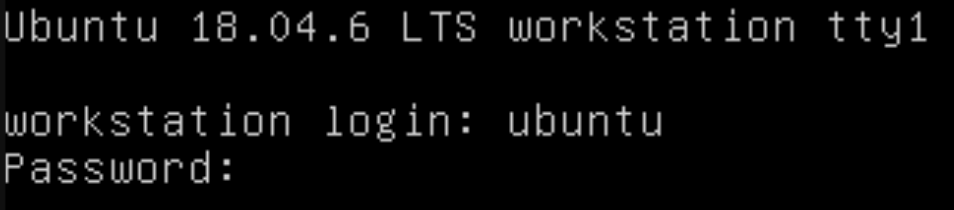
\includegraphics[scale=0.75]{images/part1/step1.png}
    \end{center}

    \item Enter the IP address of the \textbf{devstack} machine (\textbf{192.168.1.20}) into the address bar, and log
    into the OpenStack Horizon Dashboard. The username is \textbf{admin} and the password is \textbf{secret}.
    
    \begin{center}
        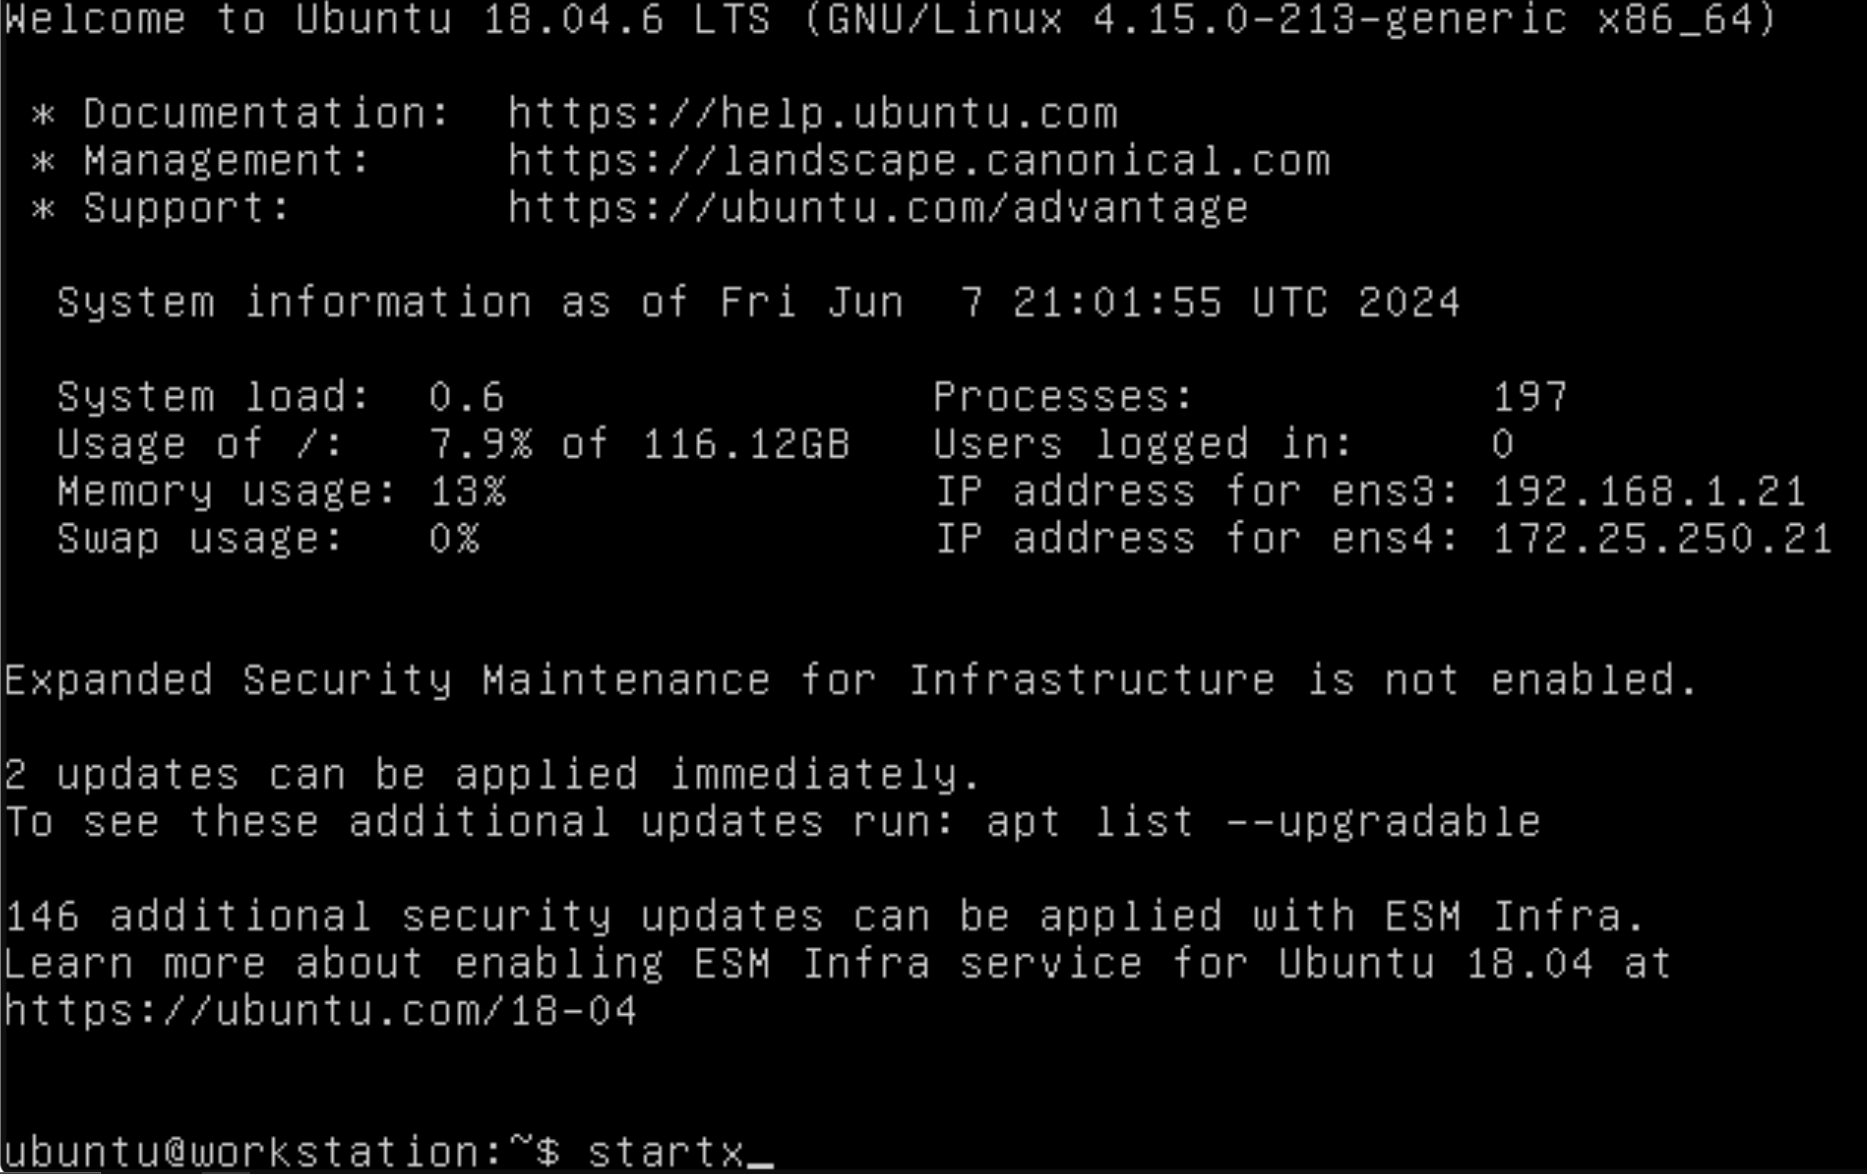
\includegraphics[scale=0.75]{images/part1/step2.png}
    \end{center}

    \item Create a project named \textbf{dev}. First, navigate to \textbf{Identity $>$ Projects}, then click on
    \textbf{Create Project}.

    \begin{center}
        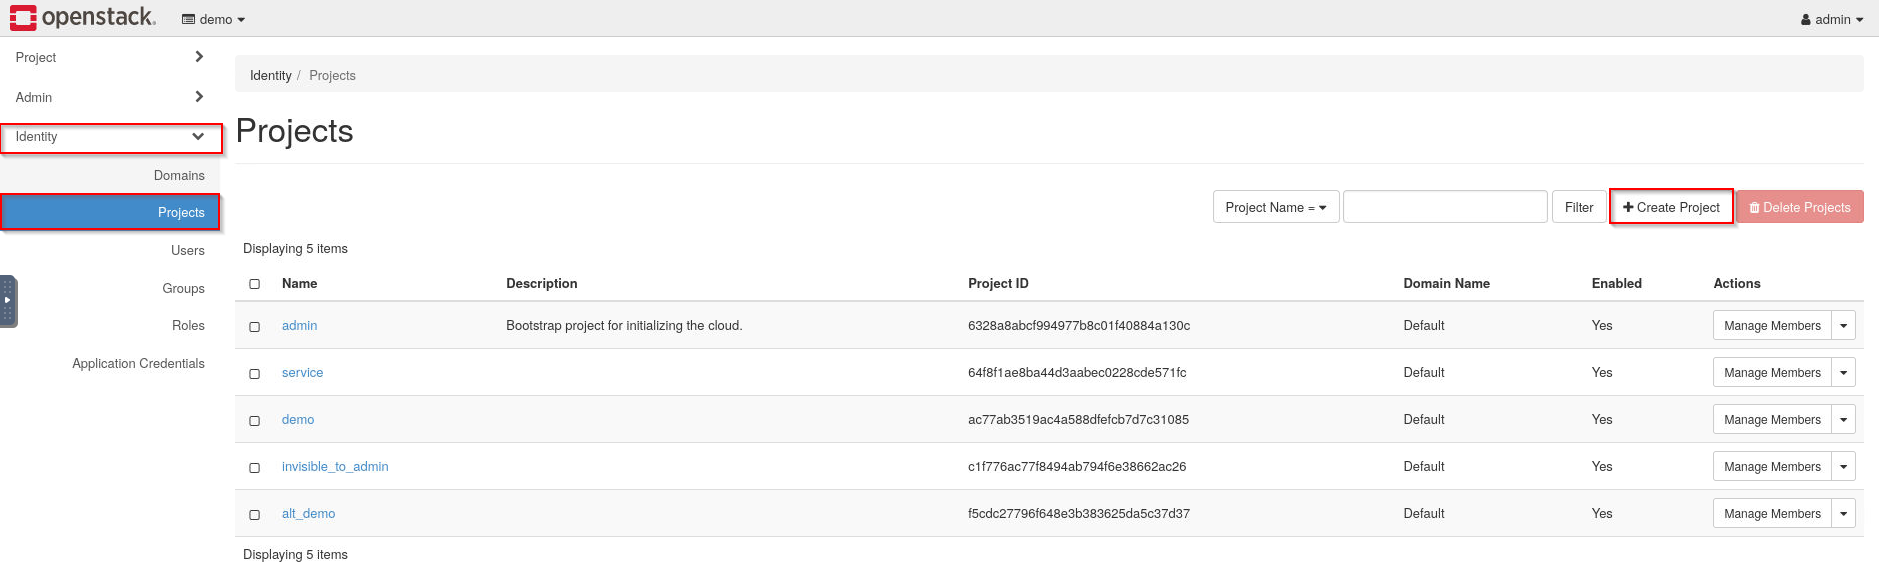
\includegraphics[width=\linewidth]{images/part1/step3.png}
    \end{center}

    \item Enter \textbf{dev} in the \textit{Name} field and \textbf{Dev Project} in the \textit{Description} field.
    Leave the \textbf{Enabled} check box selected, then click on \textbf{Create Project}.

    \begin{center}
        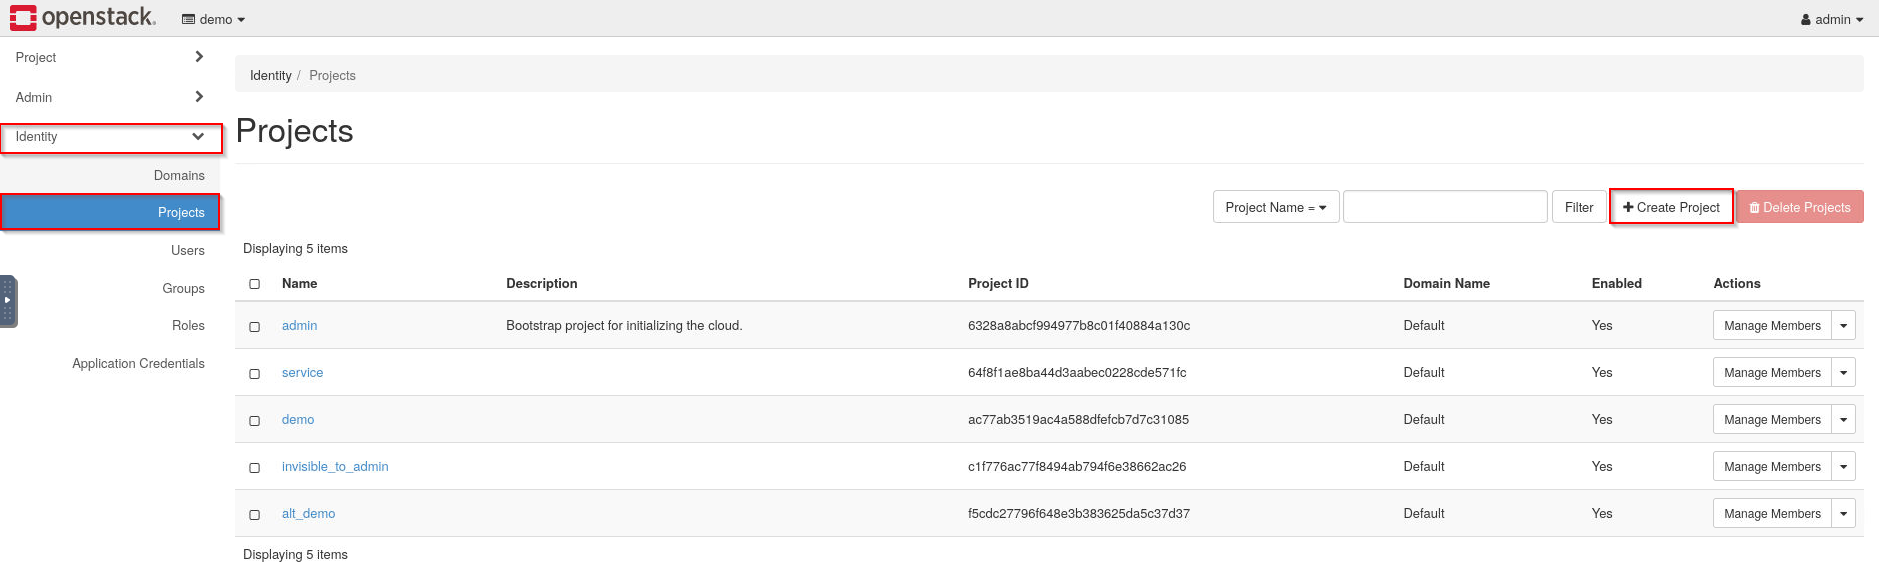
\includegraphics[width=\linewidth]{images/part1/step4.png}
    \end{center}

    \begin{notebox}
        Notice the \textbf{dev} project now appears in the \textit{Horizon Dashboard}.
    \end{notebox}

    \item Log out of the Horizon Dashboard by clicking on admin at the top right and selecting \textbf{Sign Out}.
    
    \begin{center}
        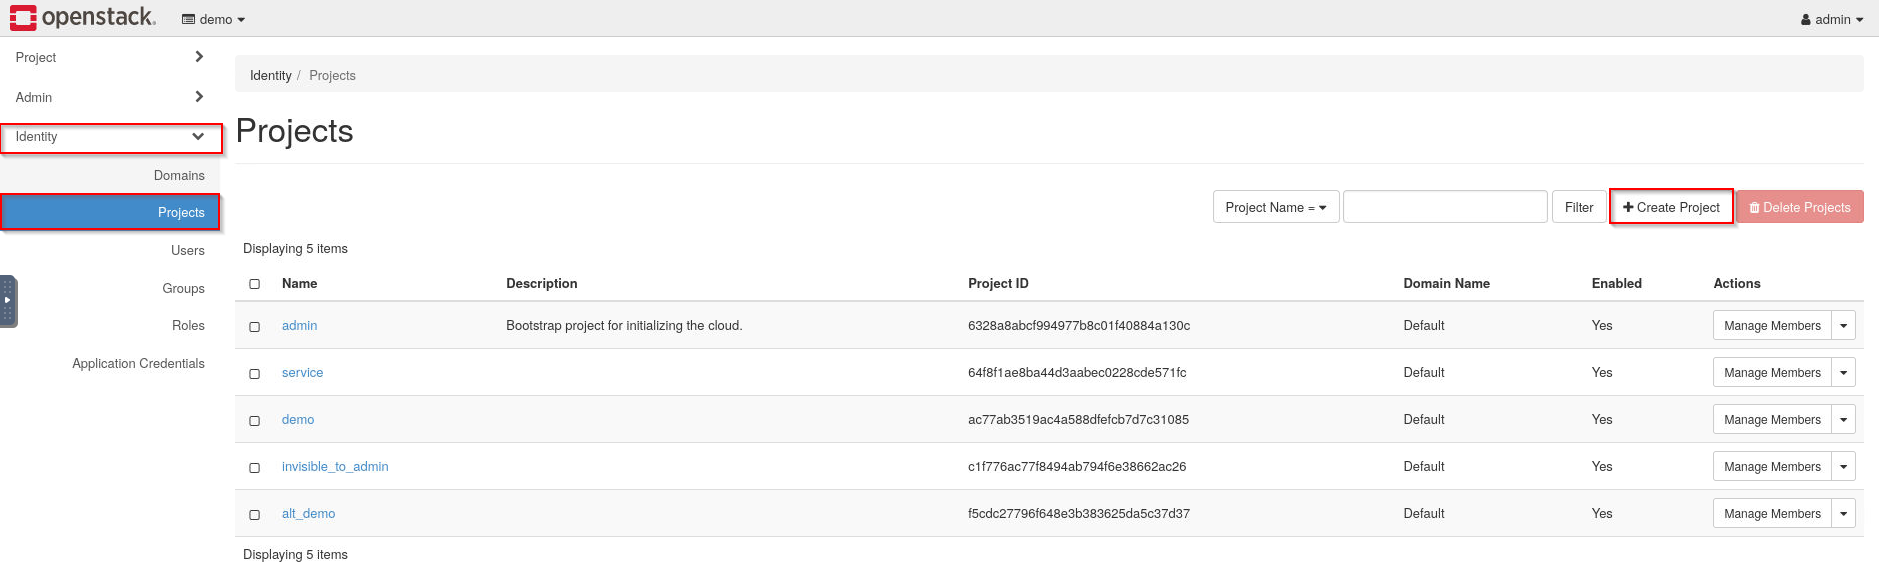
\includegraphics[scale=0.75]{images/part1/step5.png}
    \end{center}

    \item Close the web browser and continue to the next task.
\end{enumerate}

\section{Create and Delete Projects Using the OpenStack Unified CLI}
\label{sec:create_and_delete_projects_using_the_openstack_unified_cli}
In this task, you will use the \textit{OpenStack Unified CLI} to create a project from the command line.

\begin{enumerate}    
    \item Open a terminal, either by right-clicking the desktop and selecting \textbf{Open Terminal Here}, by clicking
    the terminal icon in the icon bar at the bottom of the screen, or by selecting \textbf{Applications} at the top
    left of the screen, then selecting \textbf{Terminal Emulator}.

    \begin{center}
        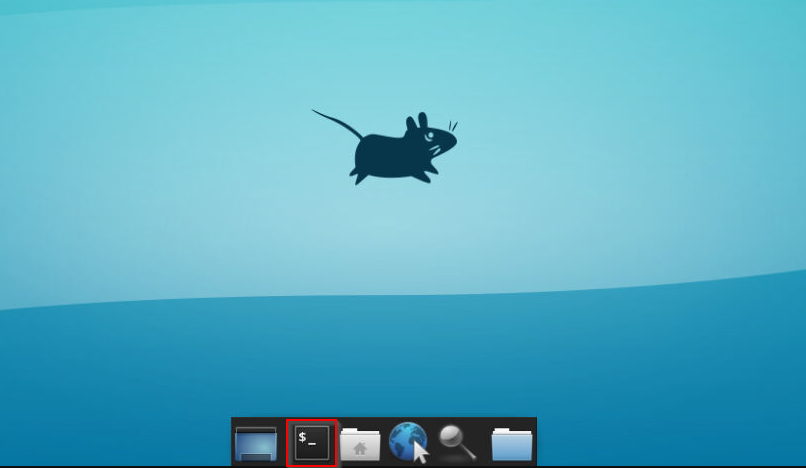
\includegraphics[width=\linewidth]{images/part2/step1.png}
    \end{center}

    \item Use the \textbf{\texttt{source}} command with the \textbf{keystonerc-admin} argument to access OpenStack
    as the admin.
\begin{lstlisting}
ubuntu@workstation:~$ source ~/keystonerc-admin
\end{lstlisting}
    
    \begin{center}
        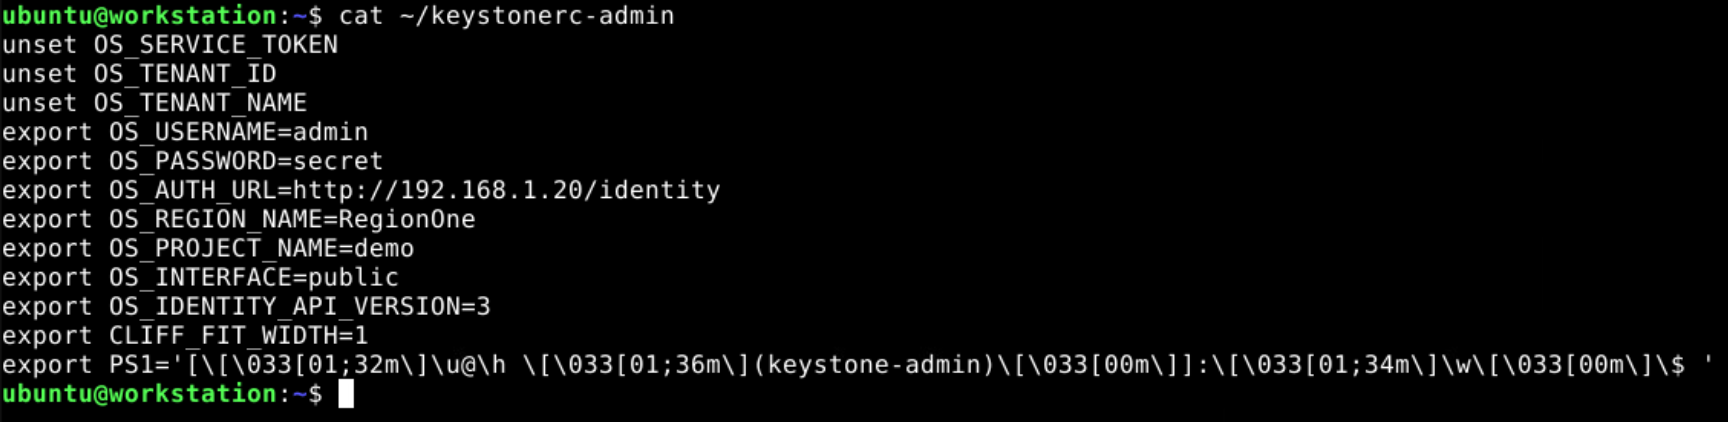
\includegraphics[width=\linewidth]{images/part2/step2.png}
    \end{center}

    \item Enter the command below to create a project named \textbf{testing}.
\begin{lstlisting}
ubuntu@workstation:~$ openstack project create \
> --description testing \
> --enable testing
\end{lstlisting}

    \begin{center}
        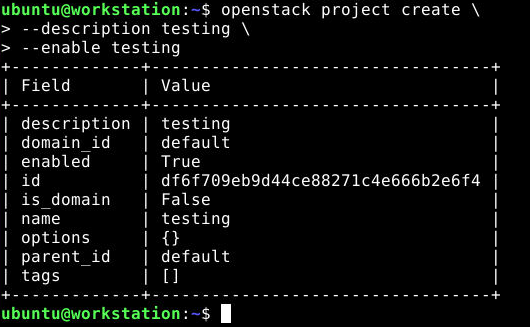
\includegraphics[width=\linewidth]{images/part2/step3.png}
    \end{center}

    \begin{tipbox}
        When typing the command make sure there is a space between \textbf{\texttt{create}} and the
        \textbf{\texttt{\textbackslash}}, and press \textbf{Enter} to get the \textbf{\texttt{>}} and continue typing
        therest of the command.
    \end{tipbox}

    \item Enter the command below to verify the project has been created.
\begin{lstlisting}
ubuntu@workstation:~$ openstack project list
\end{lstlisting}

    \begin{center}
        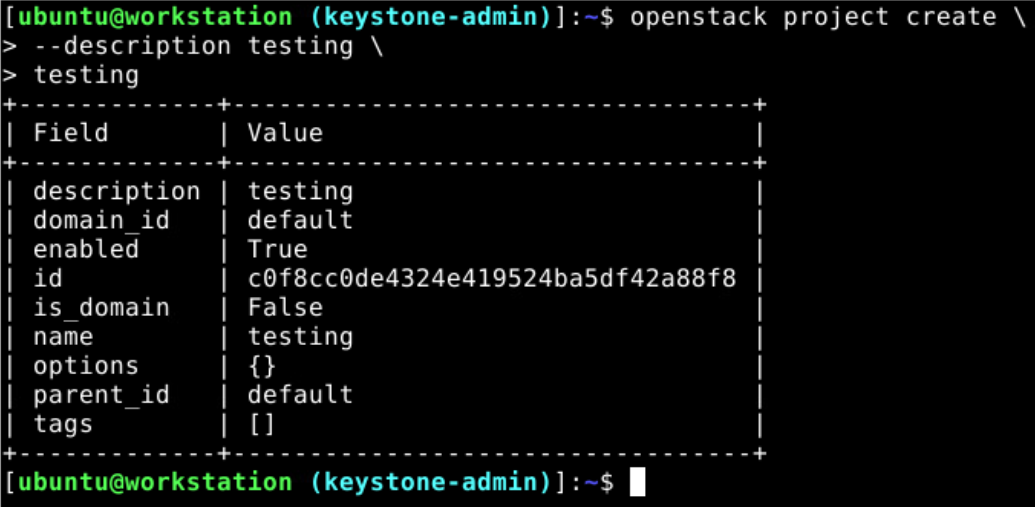
\includegraphics[width=\linewidth]{images/part2/step4.png}
    \end{center}

    \item Delete the \textbf{testing} project by entering the command below.
\begin{lstlisting}
ubuntu@workstation:~$ openstack project delete testing
\end{lstlisting}

    \begin{center}
        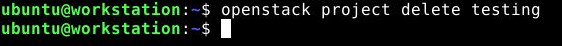
\includegraphics[width=\linewidth]{images/part2/step5.png}
    \end{center}

    \item Verify the \textbf{testing} project has been deleted by listing the projects again and noting that
    \textbf{testing} no longer appears.
\begin{lstlisting}
ubuntu@workstation:~$ openstack project list
\end{lstlisting}

    \begin{center}
        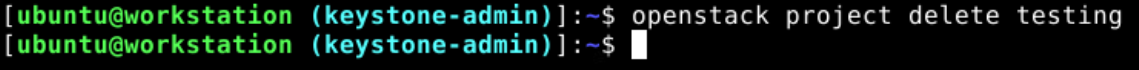
\includegraphics[width=\linewidth]{images/part2/step6.png}
    \end{center}

    \item Leave the terminal window open and continue to the next task.
\end{enumerate}

\section{Managing Users Using the Horizon Dashboard}
\label{sec:managing_users_using_the_horizon_dashboard}
In this task, you will use the \textit{Horizon Dashboard} to manage users.

\begin{enumerate}
    \item Open the web browser, navigate to the OpenStack login page at \textbf{http://192.168.1.20}, and log in with
    username \textbf{admin} and password \textbf{secret} as before. In the following steps, you will create users named
    \textbf{cloud-dev}, \textbf{cloud-test1}, and \textbf{cloud-test2}; set all of these account passwords to
    \textbf{secret}; and add these accounts to the \textbf{dev} project. 

    \item First, navigate to \textbf{Identity $>$ Users} and click on \textbf{Create User}.

    \begin{center}
        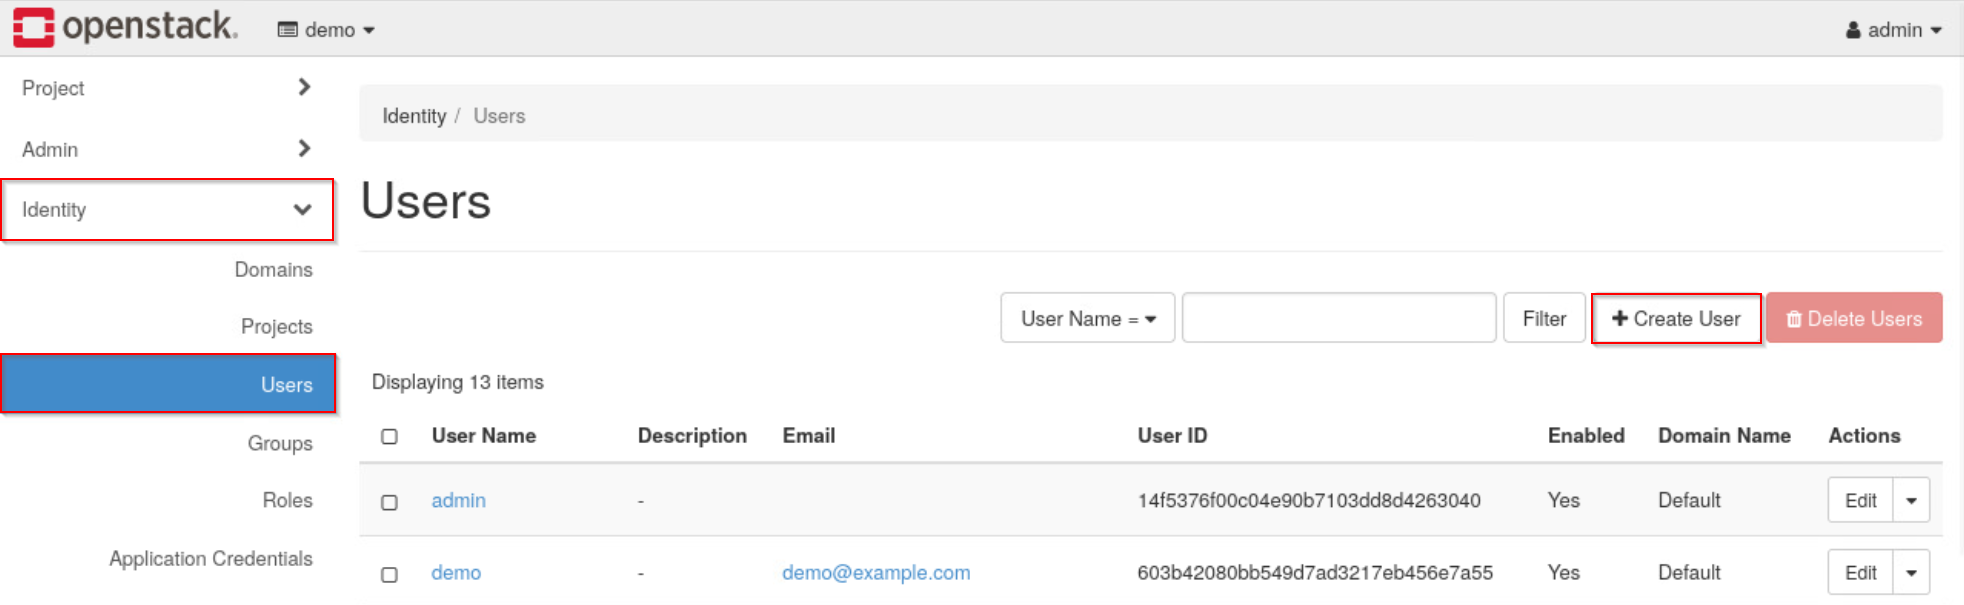
\includegraphics[width=\linewidth]{images/part3/step2.png}
    \end{center}
    
    \item In the \textit{Create User} dialog box, enter \textbf{cloud-dev} in the \textit{User Name} field, and
    \textbf{secret} in the \textit{Password} and \textit{Confirm Password} fields.

    \begin{center}
        \includegraphics[width=\linewidth]{images/part3/step3.png}
    \end{center}

    \begin{tipbox}
        You will need to use the scroll bar on the right side of the dialog box to scroll down for more fields.
    \end{tipbox}

    \item After scrolling down, select the \textbf{dev} project from the \textit{Primary Project} drop down. Leave the
    \textit{Role} set to \textbf{member}, and leave the \textbf{Enabled} check box selected. Click on
    \textbf{Create User}.

    \begin{center}
        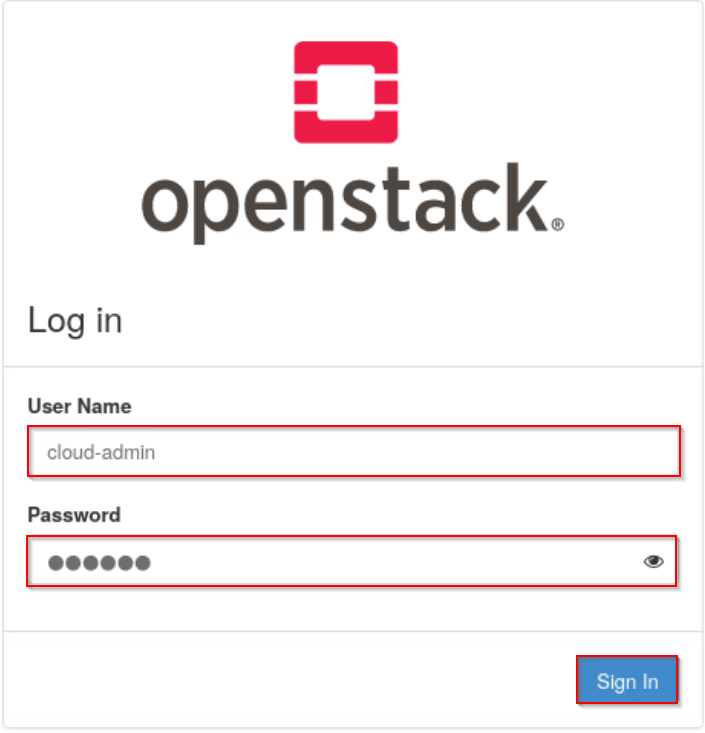
\includegraphics[width=\linewidth]{images/part3/step4.png}
    \end{center}

    \item Repeat steps 2 through 4 to create the \textbf{cloud-test1} and \textbf{cloud-test2} user accounts.

    \item Delete the \textbf{cloud-test1} user account. On the \textit{Users} tab, select the \textbf{cloud-test1} user
    account checkbox and click on \textbf{Delete Users} and then confirm the deletion in the dialog box.

    \begin{center}
        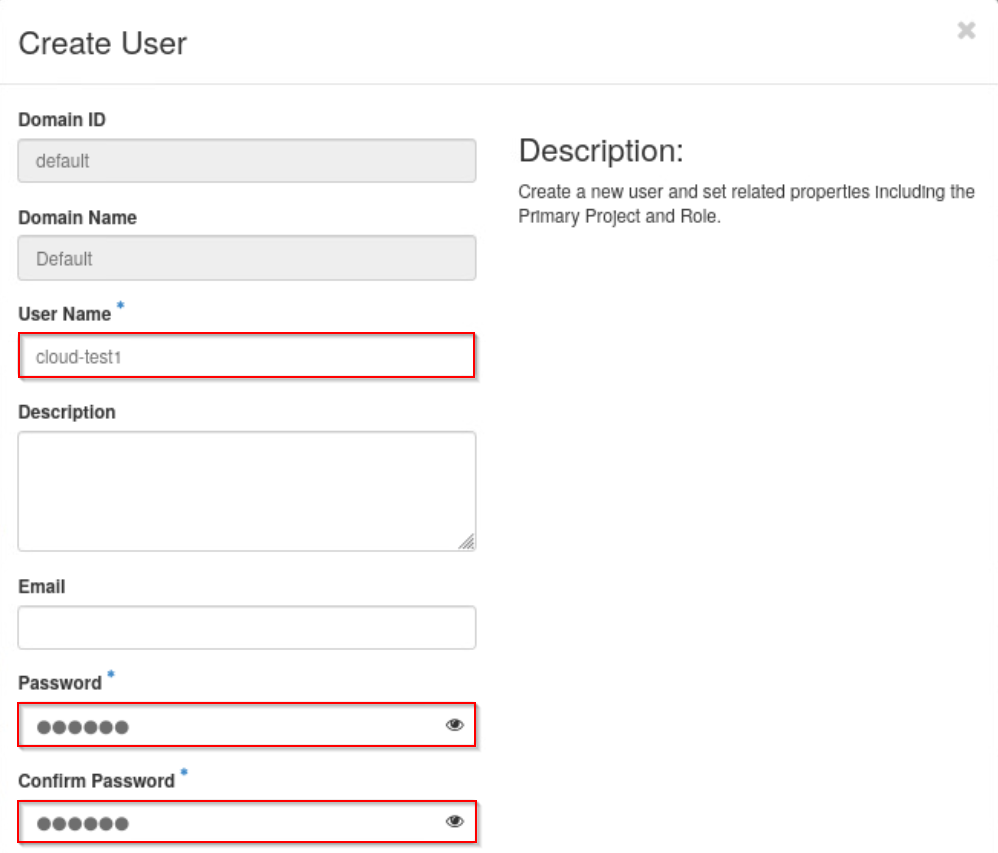
\includegraphics[width=\linewidth]{images/part3/step6.png}
    \end{center}

    \item Disable the \textbf{cloud-test2} user account. On the \textit{Users} tab, select \textbf{Disable User} under
    the \textit{Actions} column for the \textbf{cloud-test2} user account entry.

    \begin{center}
        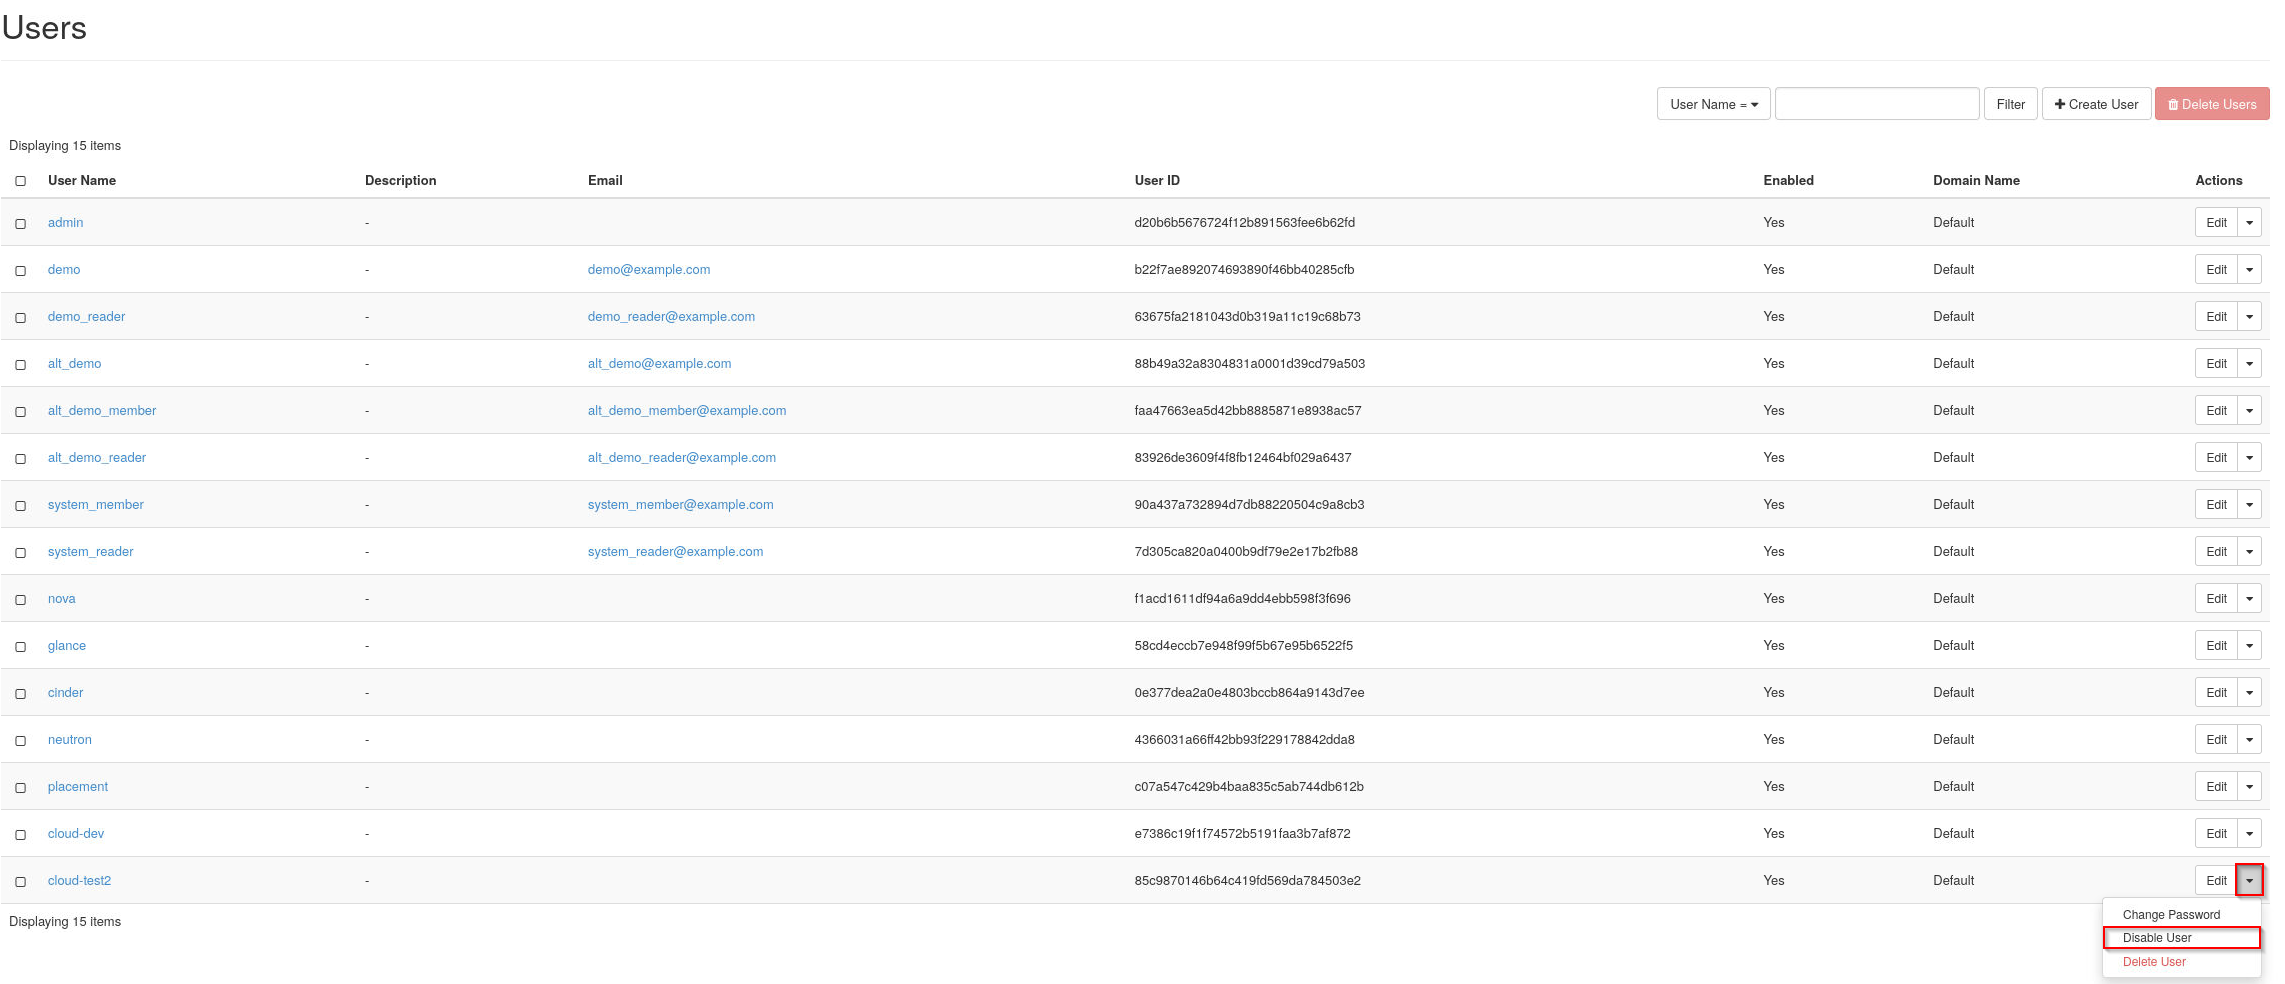
\includegraphics[width=\linewidth]{images/part3/step7.png}
    \end{center}

    \item Log out of the dashboard as \textbf{admin}. Select the \textit{admin} drop down at the top right and click on
    \textbf{Sign Out}.

    \begin{center}
        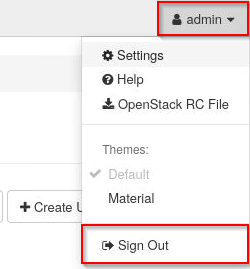
\includegraphics[scale=0.75]{images/part3/step8.png}
    \end{center}

    \item At the Horizon Dashboard screen, attempt to log in as \textbf{cloud-test2} with the password \textbf{secret}.
    
    \begin{center}
        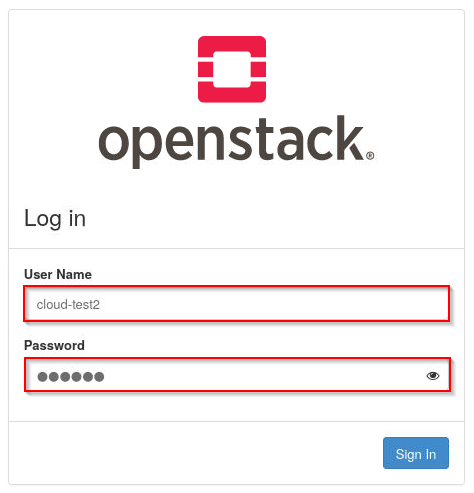
\includegraphics[scale=0.75]{images/part3/step9.png}
    \end{center}

    \begin{notebox}
        Notice the user account is disabled as intended.
    \end{notebox}

    \item Log back into the dashboard as \textbf{admin} and re-enable the \textbf{cloud-test2} user. Navigate to
    \textbf{Identity $>$ Users}. Click on the drop down in the \textit{Actions} column in the row for
    \textbf{cloud-test2} and select \textbf{Enable User}.

    \begin{center}
        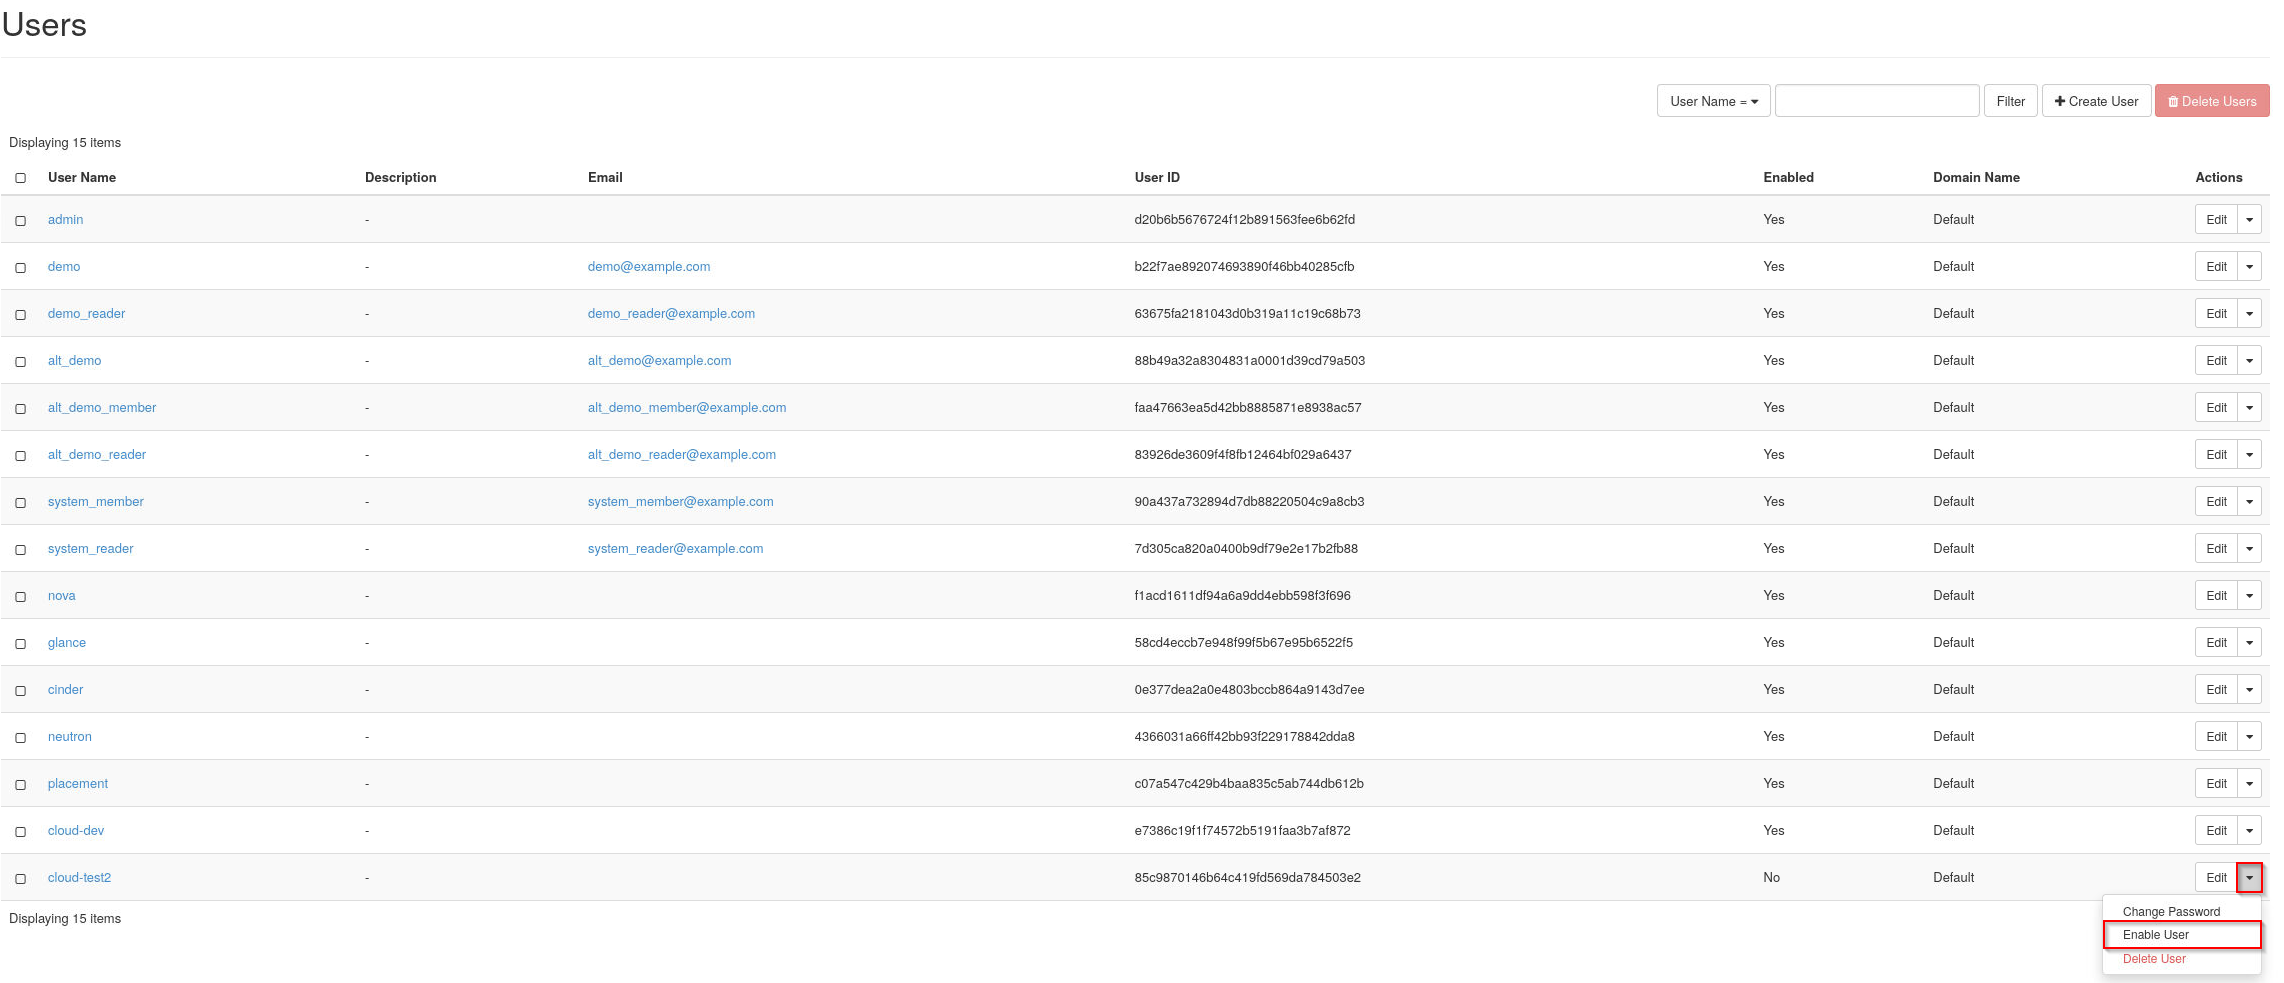
\includegraphics[width=\linewidth]{images/part3/step10.png}
    \end{center}

    \item Select the same drop down, but this time click on \textbf{Change Password}.

    \begin{center}
        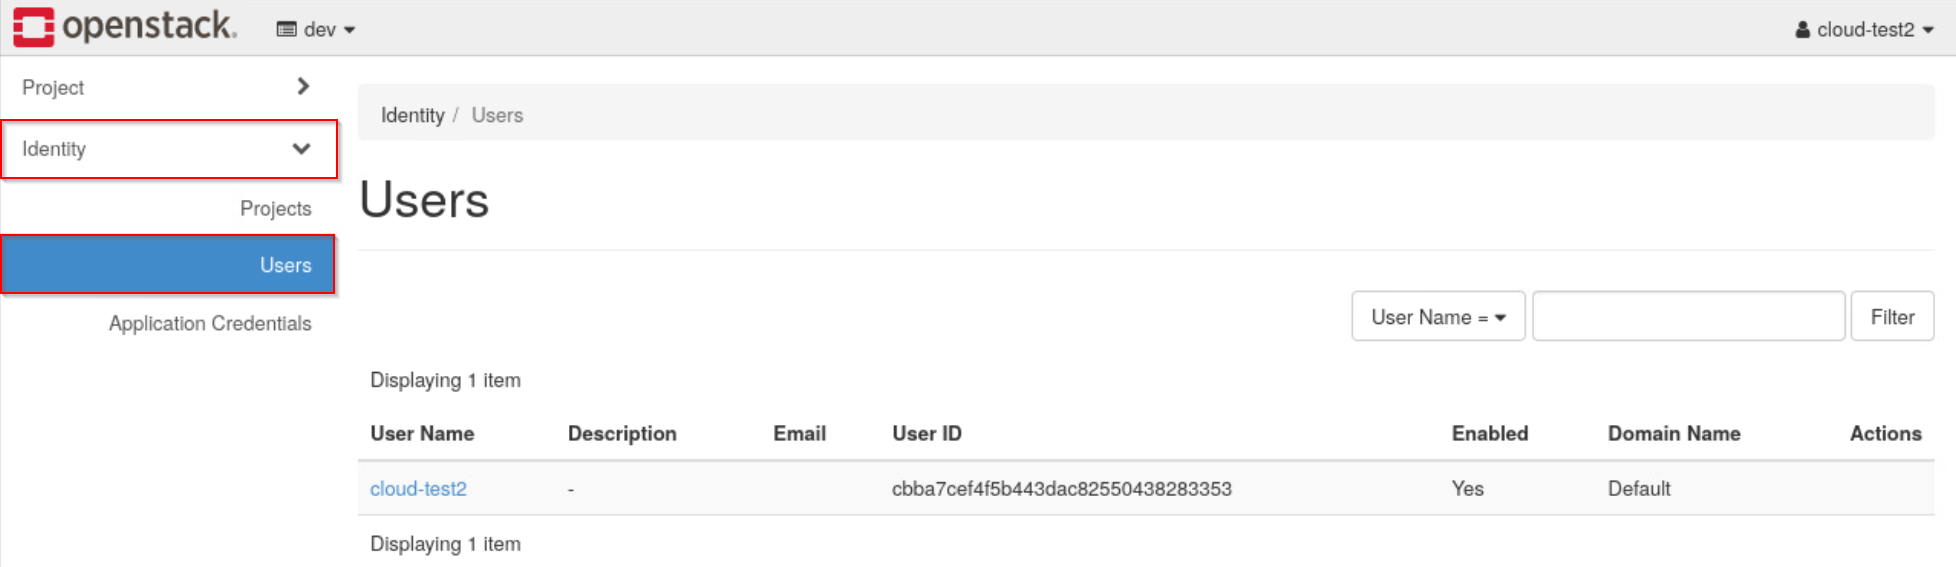
\includegraphics[width=\linewidth]{images/part3/step11.png}
    \end{center}
    
    \item Change the password for \textbf{cloud-test2} to \textbf{password}. Enter \textbf{password} into the
    \textit{Password} and \textit{Confirm Password} fields, then click on \textbf{Save}.

    \begin{center}
        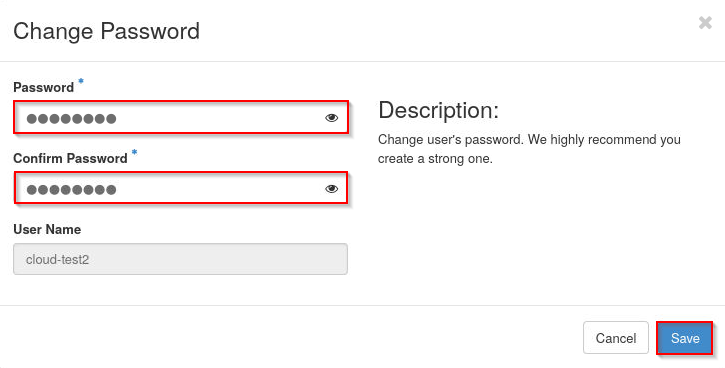
\includegraphics[width=\linewidth]{images/part3/step12.png}
    \end{center}

    \item Log out of the dashboard and log back in as \textbf{cloud-test2} with the password \textbf{password} to verify
    the password has been changed.

    \item Log out of the dashboard and close the web browser. Continue to the next task.
\end{enumerate}

\section{Managing Users Using the OpenStack Unified CLI}
\label{sec:managing_users_using_the_openstack_unified_cli}
In this task, you will manage users using the \textit{OpenStack Unified CLI}.

\begin{enumerate}
    \item Open a terminal if you do not already have one running, and navigate to the home directory.
    
    \item Source the credential for \textbf{admin} using the \textbf{keystonerc-admin} file by entering the command
    below.
\begin{lstlisting}
ubuntu@workstation:~$ source ~/keystonerc-admin
\end{lstlisting}

    \begin{center}
        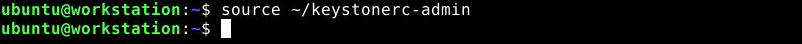
\includegraphics[width=\linewidth]{images/part4/step2.png}
    \end{center}

    \item Create the \textbf{cloud-test3} user as a member of \textbf{dev} with a password of \textbf{secret} and an
    email address of \textbf{ubuntu@workstation.lab.example.com} using the command below.
\begin{lstlisting}
ubuntu@workstation:~$ openstack user create \
> --project dev \
> --password secret \
> --email ubuntu@workstation.lab.example.com \
> cloud-test3
\end{lstlisting}

    \begin{center}
        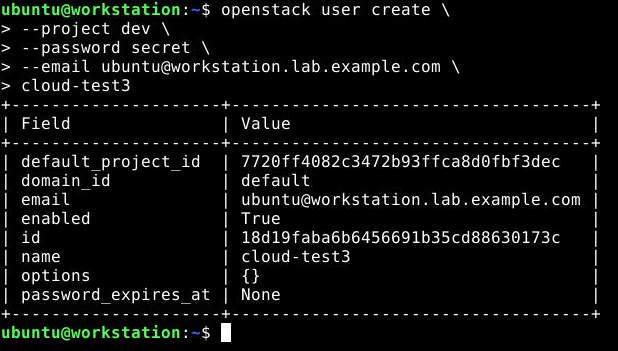
\includegraphics[width=\linewidth]{images/part4/step3.png}
    \end{center}

    \begin{tipbox}
        When typing the command, make sure there is a space between \texttt{create} and the \texttt{\textbackslash}
        character, and press \textbf{Enter} to get the \texttt{>} and continue typing the rest of the command.
    \end{tipbox}

    \item Verify the user was created using the command below.
\begin{lstlisting}
ubuntu@workstation:~$ openstack user list
\end{lstlisting}

    \begin{center}
        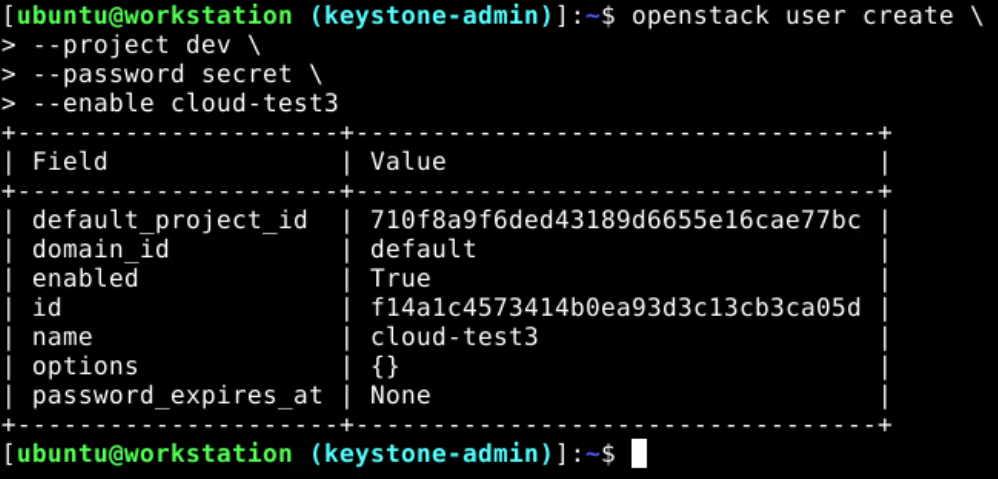
\includegraphics[width=\linewidth]{images/part4/step4.png}
    \end{center}

    \item The \textbf{cloud-test3} user will also need to be assigned a role to a project before being able to perform
    any actions. Assign a role with the command below.
\begin{lstlisting}
ubuntu@workstation:~$ openstack role add \
> --project dev \
> --user cloud-test3 \
> member
\end{lstlisting}

    \begin{center}
        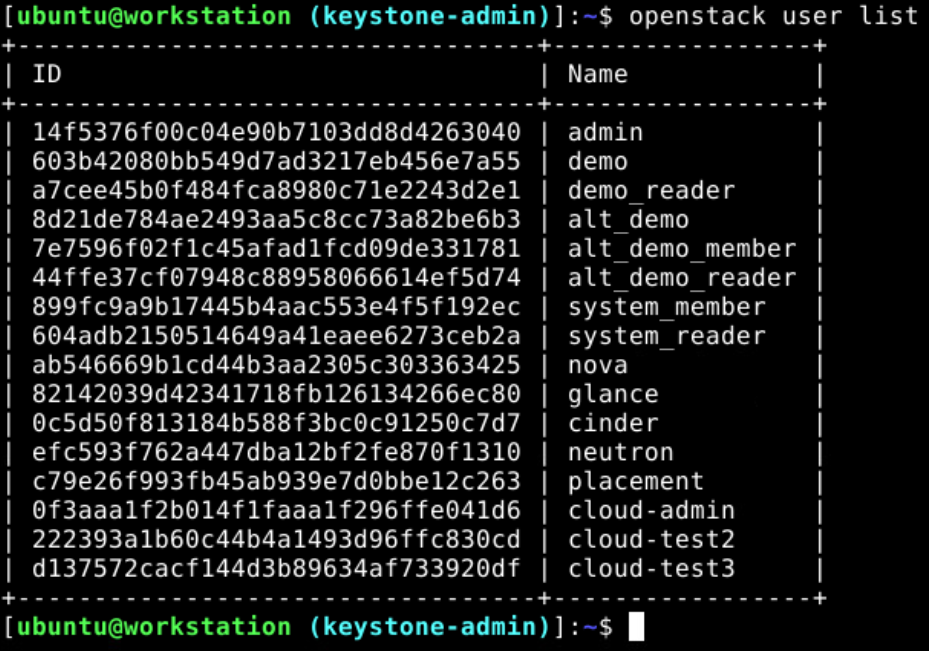
\includegraphics[width=\linewidth]{images/part4/step5.png}
    \end{center}

    \item Copy the existing \textbf{\texttildemid/keystonerc-admin} file to \textbf{\texttildemid/keystonerc-cloud-dev}
    by entering the command below.
    \label{it:copy_keystone}
\begin{lstlisting}
ubuntu@workstation:~$ cp ~/keystonerc-admin ~/keystonerc-cloud-dev
\end{lstlisting}

    \begin{center}
        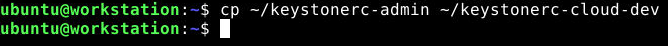
\includegraphics[width=\linewidth]{images/part4/step6.png}
    \end{center}

    \item Edit the \textbf{\texttildemid/keystonerc-cloud-dev} file and modify the \texttt{OS\_USERNAME}, \texttt{OS\_PASSWORD}, and
    \texttt{OS\_PROJECT\_NAME} using the \textbf{\texttt{nano}} command. Modify the file so the content matches below.
    When you are finished, press \textbf{CTRL+X}, then \textbf{Y} to accept the file changes. Press \textbf{Enter} to
    save and exit \textbf{\texttt{nano}}.
    \label{it:edit_keystone}
\begin{lstlisting}
ubuntu@workstation:~$ nano ~/keystonerc-cloud-dev
\end{lstlisting}

    \begin{center}
        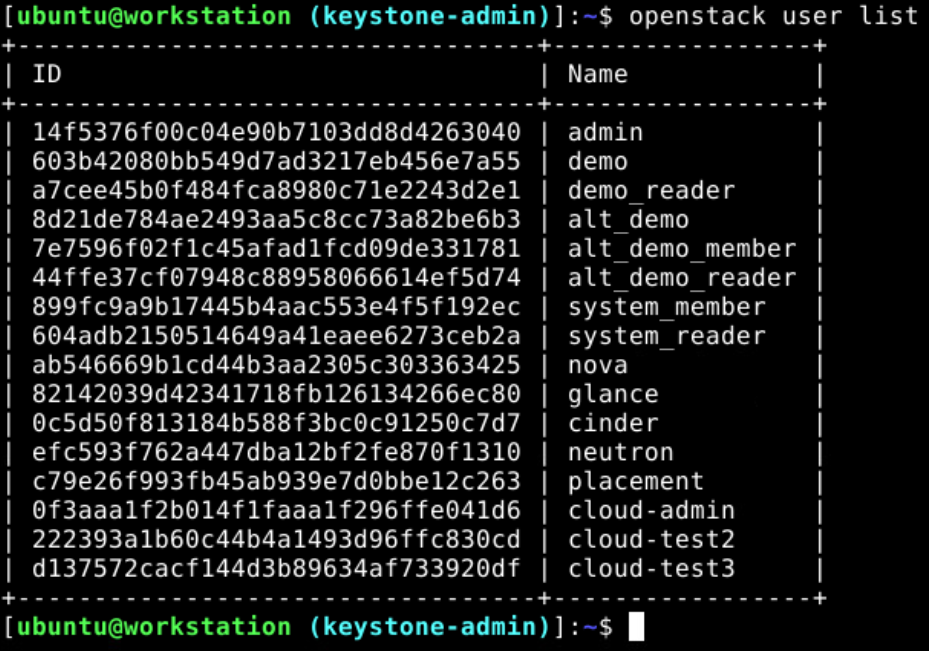
\includegraphics[width=\linewidth]{images/part4/step7.png}
    \end{center}

    \begin{tipbox}
        To avoid any confusion about which user's credentials you are currently using, you can set the \texttt{PS1}
        environment variable in the keystone file so that the terminal prompt shows the active user. For example, the
        line \texttt{export PS1='[\textbackslash u@\textbackslash h \textbackslash W(keystone-cloud-dev)]\$ '} will
        make the terminal prompt appear as \texttt{[ubuntu@workstation \texttildemid(keystone-cloud-dev)]\$}.
    \end{tipbox}

    \item Repeat steps \ref{it:copy_keystone} and \ref{it:edit_keystone}, this time for user \textbf{cloud-test3}.
    
    \item Disable the \textbf{cloud-test3} account by entering the command below
\begin{lstlisting}
ubuntu@workstation:~$ openstack user set \
> --disable cloud-test3
\end{lstlisting}

    \begin{center}
        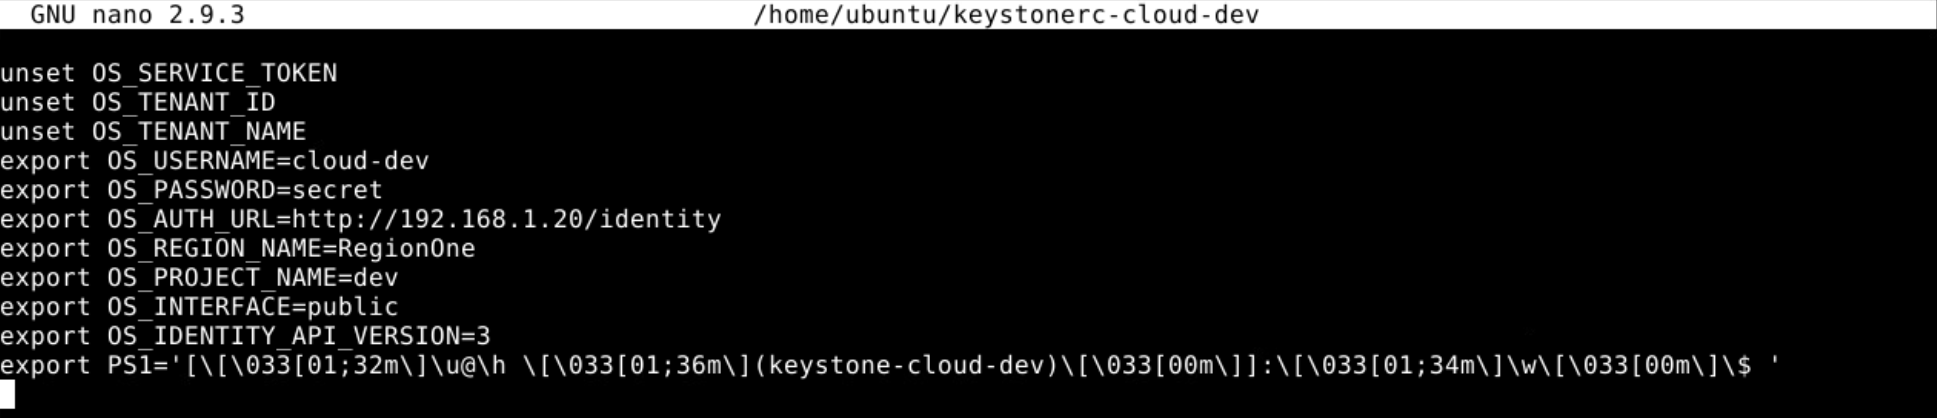
\includegraphics[width=\linewidth]{images/part4/step9.png}
    \end{center}

    \item To verify that the \textbf{cloud-test3} account is disabled, first source the
    \textbf{\texttildemid/keystonerc-cloud-test3} keystone credentials file for the \textbf{cloud-test3} user by
    entering the command below.
\begin{lstlisting}
ubuntu@workstation:~$ source ~/keystonerc-cloud-test3
\end{lstlisting}

    \begin{center}
        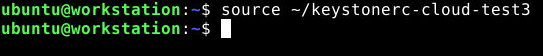
\includegraphics[width=\linewidth]{images/part4/step10.png}
    \end{center}

    \item Now try listing a flavor by running the command below and take note of the response.
\begin{lstlisting}
ubuntu@workstation:~$ openstack flavor list
\end{lstlisting}

    \begin{center}
        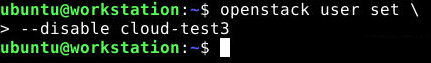
\includegraphics[width=\linewidth]{images/part4/step11.png}
    \end{center}

    \item Source the keystone credentials using the \textbf{admin} user keystone file so that further changes can be
    made to the accounts.
\begin{lstlisting}
ubuntu@workstation:~$ source ~/keystonerc-admin
\end{lstlisting}

    \begin{center}
        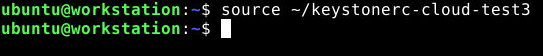
\includegraphics[width=\linewidth]{images/part4/step12.png}
    \end{center}

    \item Enable the \textbf{cloud-test3} user account, change the password to \textbf{password}, and change the email
    address to \textbf{ubuntu@devstack.lab.example.com}.    
\begin{lstlisting}
openstack user set \
> --password password \
> --email ubuntu@devstack.lab.example.com \
> --enable cloud-test3
\end{lstlisting}

    \begin{center}
        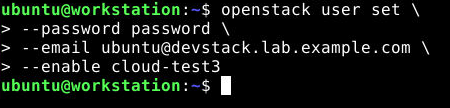
\includegraphics[width=\linewidth]{images/part4/step13.png}
    \end{center}

    \item Set the password, \textbf{password} in the keystone credential file for \textbf{cloud-test3}. Modify the file
    so the content matches below. When you are finished, press \textbf{CTRL+X}, then \textbf{Y} to accept the file
    changes. Press \textbf{Enter} to save and exit \textbf{\texttt{nano}}.
\begin{lstlisting}
ubuntu@workstation:~$ nano ~/keystonerc-cloud-test3
\end{lstlisting}

    \begin{center}
        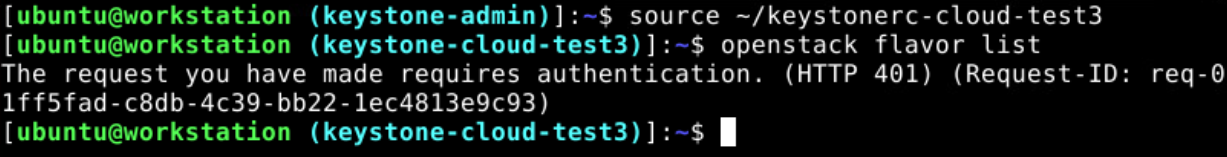
\includegraphics[width=\linewidth]{images/part4/step14.png}
    \end{center}

    \item Source the \textbf{\texttildemid/keystonerc-cloud-test3} keystone credentials file for the
    \textbf{cloud-test3} user.
\begin{lstlisting}
ubuntu@workstation:~$ source ~/keystonerc-cloud-test3
\end{lstlisting}

    \begin{center}
        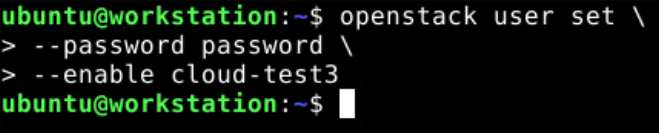
\includegraphics[width=\linewidth]{images/part4/step15.png}
    \end{center}

    \item Now that the \textbf{cloud-test3} user has been enabled, verify that the \textbf{\texttt{openstack flavor
    list}} command returns a list of available flavors.
\begin{lstlisting}
ubuntu@workstation:~$ openstack flavor list
\end{lstlisting}

    \begin{center}
        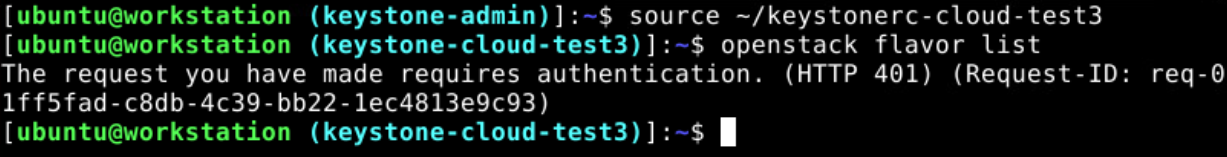
\includegraphics[width=\linewidth]{images/part4/step16.png}
    \end{center}

    \item Source the keystone credentials file for the \textbf{admin} user.
\begin{lstlisting}
ubuntu@workstation:~$ source ~/keystonerc-admin
\end{lstlisting}

    \begin{center}
        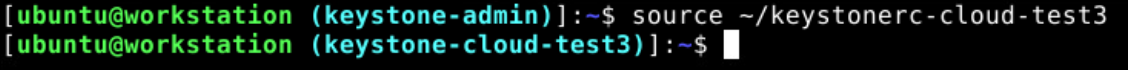
\includegraphics[width=\linewidth]{images/part4/step17.png}
    \end{center}

    \item Delete the \textbf{cloud-test2} and \textbf{cloud-test3} user accounts.
\begin{lstlisting}
ubuntu@workstation:~$ openstack user delete cloud-test2
ubuntu@workstation:~$ openstack user delete cloud-test3
\end{lstlisting}

    \begin{center}
        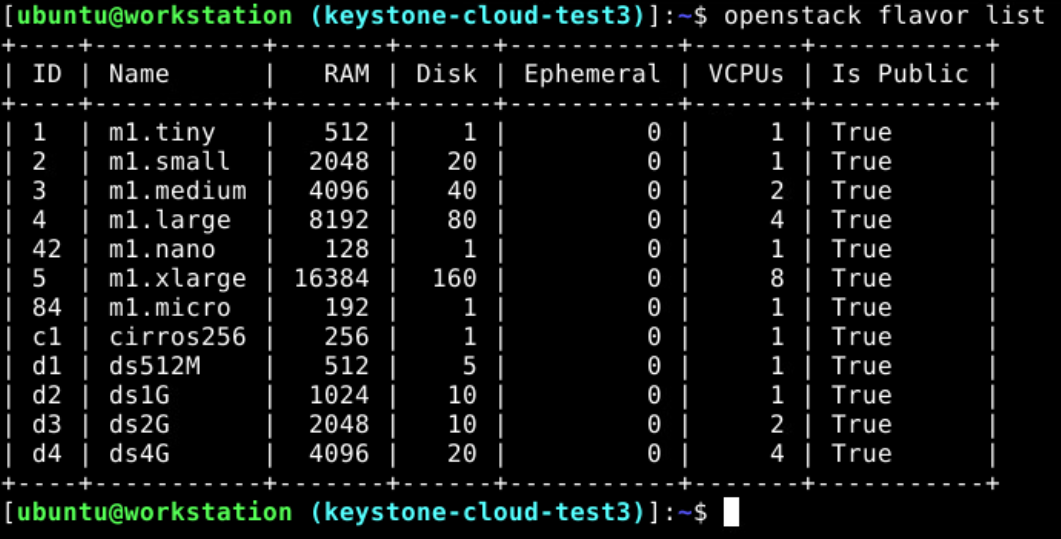
\includegraphics[width=\linewidth]{images/part4/step18.png}
    \end{center}

    \item Verify that the users have been deleted.
\begin{lstlisting}
ubuntu@workstation:~$ openstack user list
\end{lstlisting}

    \begin{center}
        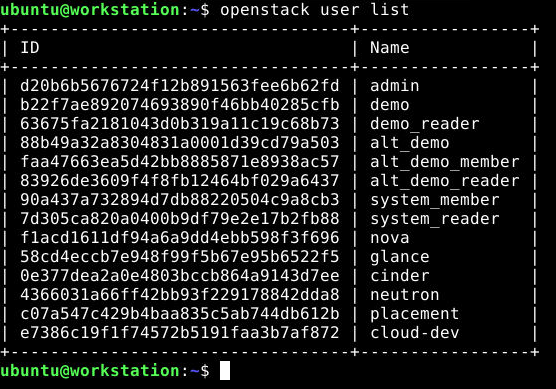
\includegraphics[width=\linewidth]{images/part4/step19.png}
    \end{center}

    \item Leave the terminal window open and continue on to the next task.
\end{enumerate}

\section{Assigning User Roles and Privileges Using the Horizon Dashboard}
\label{sec:assigning_user_roles_and_privileges_using_the_horizon_dashboard}
In this task, you will assign user roles privileges using the \textit{Horizon Dashboard}.

\begin{enumerate}
    \item Open the web browser, navigate to the OpenStack login page at \textbf{2}, and log in with username
    \textbf{admin} and password \textbf{secret} as before.

    \item Navigate to \textbf{Identity $>$ Users} and click on the \textbf{Create User} button.
    
    \begin{center}
        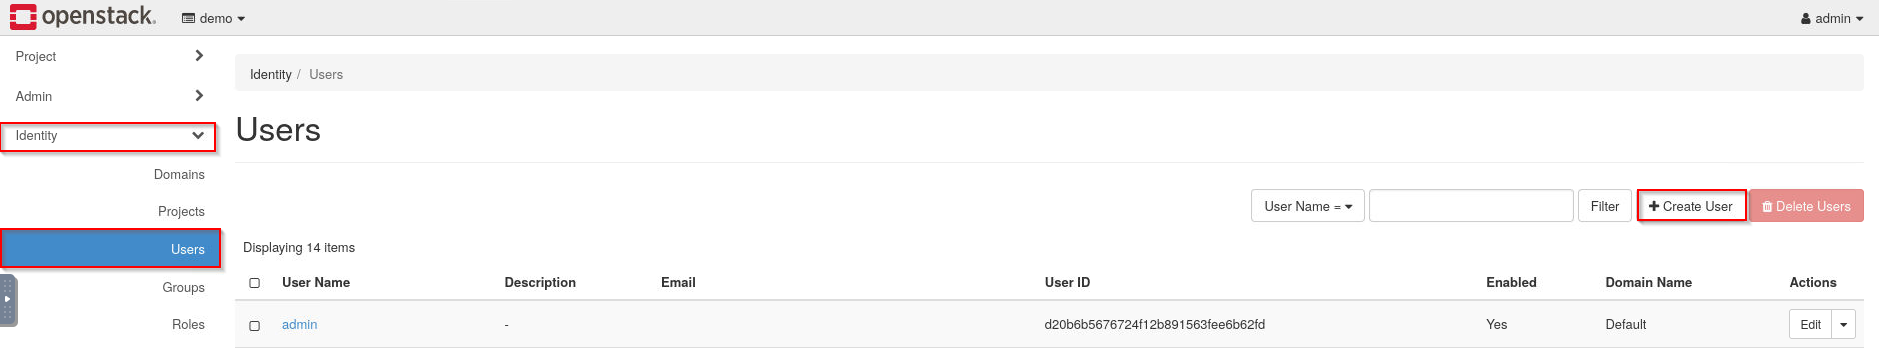
\includegraphics[width=\linewidth]{images/part5/step2.png}
    \end{center}

    \item Create the \textbf{cloud-admin} user with \textbf{admin} privileges. In the dialog box, enter
    \textbf{cloud-admin} in the \textit{User Name} field, and enter \textbf{secret} in the \textit{Password} and
    \textit{Confirm Password} fields. Select the \textbf{dev} project from the \textit{Primary Project} dropdown, and
    select \textbf{admin} in the \textit{Role} dropdown. Finally, leave the \textbf{Enabled} checkbox selected and click
    the \textbf{Create User} button.

    \begin{center}
        \includegraphics[width=\linewidth]{images/part5/step3.png}
    \end{center}

    \begin{tipbox}
        You may need to use the scroll bar on the right of the dialog to scroll down to see the projects and roles.
    \end{tipbox}

    \item Log out of the dashboard by clicking the \textbf{admin} drop down in the top right corner, then clicking
    \textbf{Sign Out}, and log back into the dashboard as the newly created \textbf{cloud-admin} user with password
    \textbf{secret}.

    \item Verify that the \textbf{cloud-admin} user has \textbf{admin} privileges by creating a user named
    \textbf{cloud-user1}. Navigate to \textbf{Identity $>$ Users} and click on the \textbf{Create User} button
    as before. In the dialog box, enter \textbf{cloud-user1} in the \textit{User Name} field and \textbf{secret} in the
    \textit{Password} and \textit{Confirm Password} fields. Select the \textbf{dev} project from the \textit{Primary
    Project} dropdown, leave the \textit{Role} set to \textbf{member}, and leave the \textbf{Enabled} checkbox
    selected. Click the \textbf{Create User} button.

    \begin{center}
        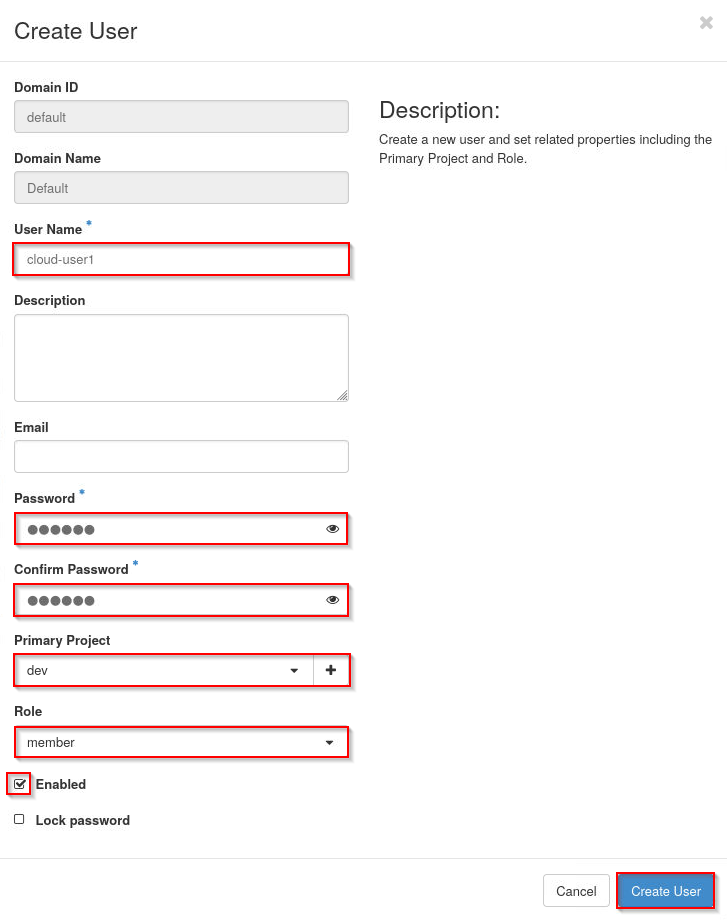
\includegraphics[width=\linewidth]{images/part5/step5.png}
    \end{center}

    \begin{tipbox}
        You may need to use the scroll bar on the right of the dialog to scroll down to see the projects and roles.
    \end{tipbox}

    \begin{center}
        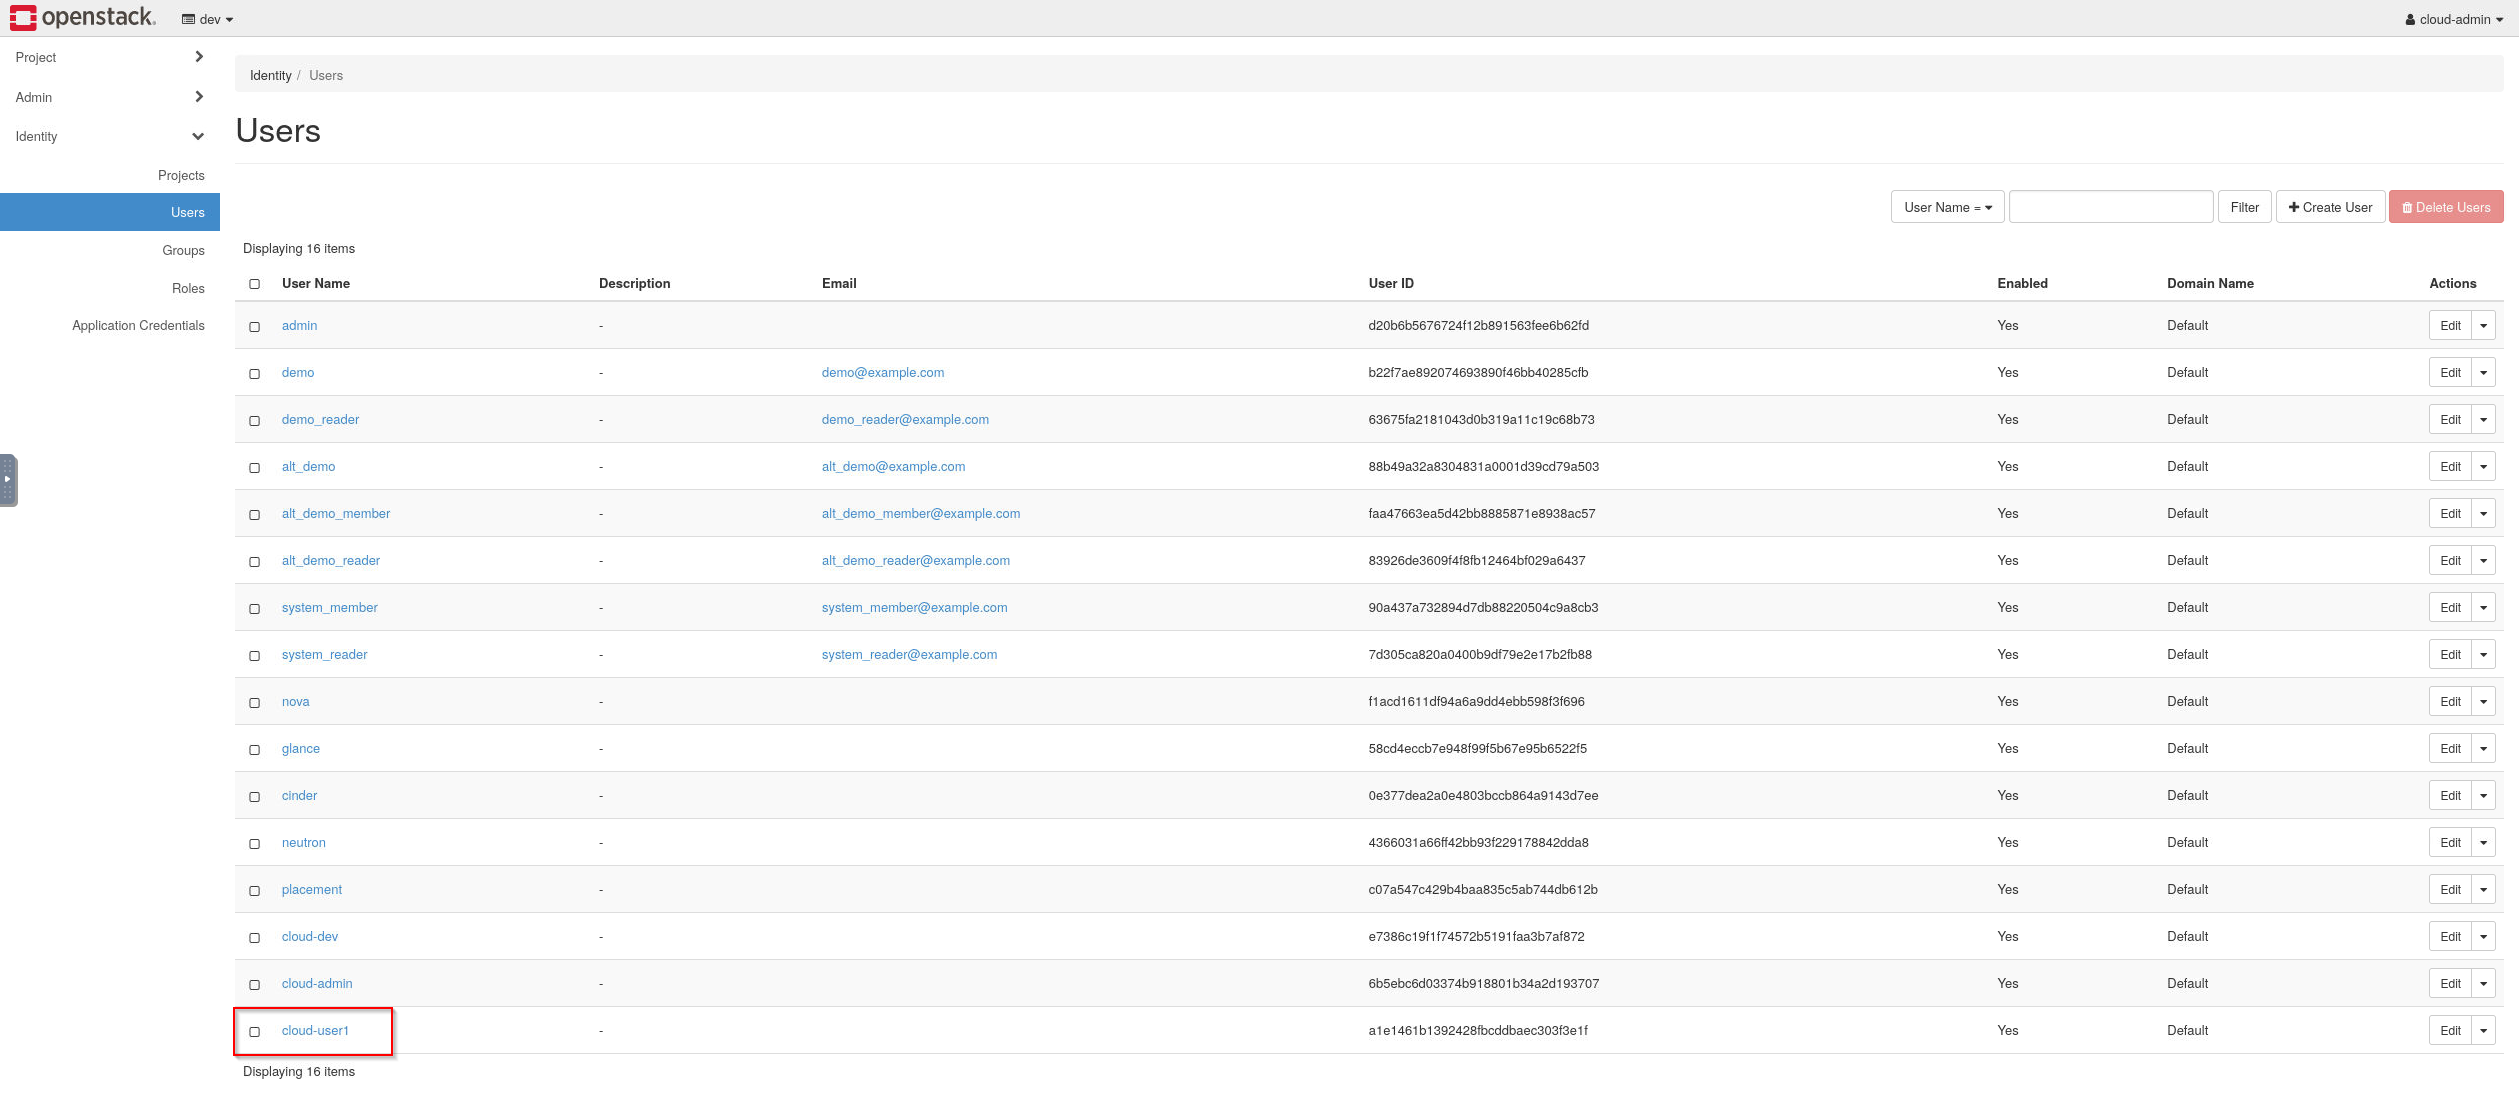
\includegraphics[width=\linewidth]{images/part5/step6.png}
    \end{center}

    \item Verify that the \textbf{cloud-user1} account appears in the user list.
    
    \item Log out of the dashboard, close the web browser, and continue to the next task.
\end{enumerate}

\section{Assigning User Roles and Privileges Using the OpenStack Unified CLI}
\label{sec:assigning_user_roles_and_privileges_using_the_openstack_unified_cli}
In this task, you will assign user roles and privileges using the \textit{OpenStack Unified CLI}.

\begin{enumerate}
    \item Open a terminal window if one is not already running.
    
    \item Source the \textbf{\texttildemid/keystonerc-admin} keystone credentials file for the
    \textbf{admin} user by entering the command below.
\begin{lstlisting}
ubuntu@workstation:~$ source ~/keystonerc-admin
\end{lstlisting}

    \begin{center}
        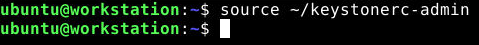
\includegraphics[width=\linewidth]{images/part6/step2.png}
    \end{center}

    \item Create the user \textbf{cloud-user2} with the password \textbf{secret}, and make it a member of the
    \textbf{dev} project.
\begin{lstlisting}
ubuntu@workstation:~$ openstack user create \
> --password secret \
> --project dev \
> cloud-user2
\end{lstlisting}

    \begin{center}
        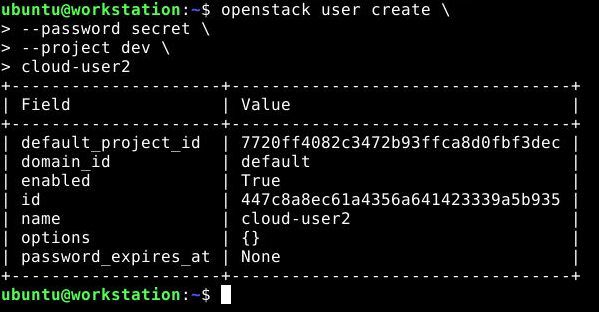
\includegraphics[width=\linewidth]{images/part6/step3.png}
    \end{center}

    \item The user \textbf{cloud-user2} is not assigned a role by default and must be assigned one. Assign the
    \textbf{admin} user role to the \textbf{cloud-user2} user.
\begin{lstlisting}
ubuntu@workstation:~$ openstack role add \
> --user cloud-user2 \
> --project dev \
> admin
\end{lstlisting}

    \begin{center}
        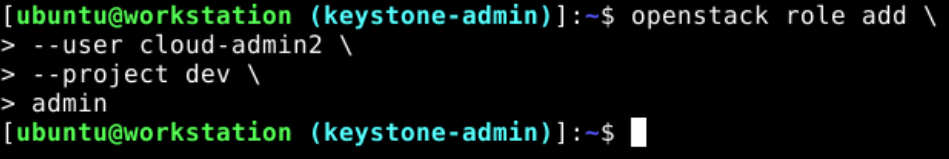
\includegraphics[width=\linewidth]{images/part6/step4.png}
    \end{center}

    \item Verify that the \textbf{cloud-user2} is in the \textbf{admin} user role for the \textbf{dev} project.
\begin{lstlisting}
ubuntu@workstation:~$ openstack role assignment list \
> --user cloud-user2 \
> --project dev \
> --names
\end{lstlisting}

    \begin{center}
        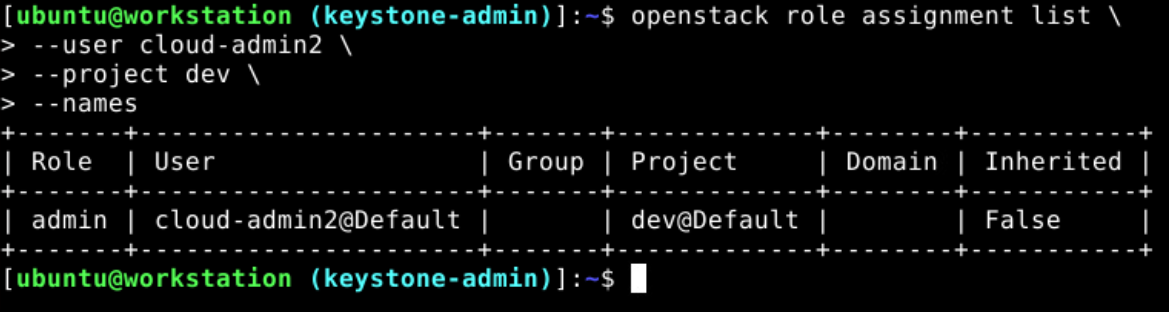
\includegraphics[width=\linewidth]{images/part6/step5.png}
    \end{center}

    \item Next, the admin role for \textbf{cloud-user2} will be used to perform an admin action. First, follow steps
    \ref{it:copy_keystone} and \ref{it:edit_keystone} from Section
    \ref{sec:managing_users_using_the_openstack_unified_cli} to create the \textbf{\texttildemid/keystonerc-cloud-user2}
    keystone credentials file for the \textbf{cloud-user2} user.

    \item Source the \textbf{\texttildemid/keystonerc-cloud-user2} keystone credentials file for the
    \textbf{cloud-user2} user.
\begin{lstlisting}
ubuntu@workstation:~$ source ~/keystonerc-cloud-user2
\end{lstlisting}

    \begin{center}
        \includegraphics[width=\linewidth]{images/part6/step7.png}
    \end{center}

    \item Delete the \textbf{cloud-user1} user.
\begin{lstlisting}
ubuntu@workstation:~$ openstack user delete cloud-user1
\end{lstlisting}

    \begin{center}
        \includegraphics[width=\linewidth]{images/part6/step8.png}
    \end{center}

    \item Delete the \textbf{cloud-user2} user.
\begin{lstlisting}
ubuntu@workstation:~$ openstack user delete cloud-user2
\end{lstlisting}    

    \begin{center}
        \includegraphics[width=\linewidth]{images/part6/step9.png}
    \end{center}

    \item Since the \textbf{cloud-user2} user has been deleted, the keystone credentials no longer authenticate the
    user. You can verify this by attempting to list OpenStack users.
\begin{lstlisting}
ubuntu@workstation:~$ openstack user list
\end{lstlisting}

    \begin{center}
        \includegraphics[width=\linewidth]{images/part6/step10.png}
    \end{center}

    \item Source the \textbf{\texttildemid/keystonerc-admin} keystone credentials file for the \textbf{cloud-admin}
    user.
\begin{lstlisting}
ubuntu@workstation:~$ source ~/keystonerc-admin
\end{lstlisting}

    \begin{center}
        \includegraphics[width=\linewidth]{images/part6/step11.png}
    \end{center}

    \item Verify that the \textbf{cloud-user1} and \textbf{cloud-user2} users have been deleted.
\begin{lstlisting}
ubuntu@workstation:~$ openstack user list
\end{lstlisting}

    \begin{center}
        \includegraphics[width=\linewidth]{images/part6/step12.png}
    \end{center}

    \item Source the \textbf{\texttildemid/keystonerc-cloud-dev} keystone credentials for the \textbf{cloud-dev} user and
    attempt to list the users. Notice the error displayed when a non-privileged user runs a command that requires
    administrator privileges.
\begin{lstlisting}
ubuntu@workstation:~$ openstack user list
\end{lstlisting}

    \begin{center}
        \includegraphics[width=\linewidth]{images/part6/step13.png}
    \end{center}

    \item The lab is now complete.

\end{enumerate}
\end{document}
